\chapter[Appendix to VAE-SNE]{Appendix to ``VAE-SNE: a deep generative model for simultaneous dimensionality reduction and clustering"}
\newpage

\begin{table}[!htb]
\caption{  \textbf{Ranked information preservation metric performance for nonlinear dimension reduction algorithms}.
Rankings for each nonlinear dimension reduction algorithm in terms of general performance for local, global, fine-scale, and temporal structure preservation (lower is better).}
\resizebox{\linewidth}{!}{
\begin{tabular}{llllll}
\textbf{name}            & \textbf{citation} & \textbf{local} & \textbf{global} & \textbf{fine-scale} & \textbf{temporal} \\
VAE-SNE (t-SNE) & this paper            &  1 & 1 & 2 & 2 \\
VAE-SNE (SNE)   & this paper            & 2 &  1 & 2 &  1 \\
FIt-SNE         & Linderman et al. (2017) &  1 & 2 &  1 & 2 \\
Barnes-Hut-SNE & van der Maaten (2014) &  1               & 2                &  1                    & 2                  \\
UMAP (LE init)            & McInnes et al. (2018)   &  1 & 3 & 2 & 3 \\
UMAP (PCA init)            & McInnes et al. (2018)   &  1 & 2 & 2 & 3 \\
scvis           & Ding et al. (2018)     & 2 &  1 & 2 & 2 \\
ivis            & Szubert et al. (2019)   & 2 &  1 & 3 &  1 \\
\end{tabular}
}
\label{table:info}

\end{table}

\begin{table}[!htb]
\caption{  \textbf{Ranked processing speed performance for nonlinear dimension reduction algorithms}. Rankings for each nonlinear dimension reduction algorithm in terms of general performance for training time and test time (lower is better), as well as whether or not test time increases as a function of training set size.}
\resizebox{\linewidth}{!}{
\begin{tabular}{lllll}
\textbf{name}            & \textbf{citation}                  & \textbf{train time} & \textbf{test time} & \textbf{test time $\propto$ train size} \\
VAE-SNE         & this paper                 & 4          & 1         & no                           \\
FIt-SNE         & Linderman et al. (2017)      & 2          & 4         & no                           \\
Barnes-Hut-SNE  & van der Maaten (2014) & 3          & 5         & yes                          \\
UMAP            & McInnes et al. (2018)        & 1          & 3         & yes                          \\
scvis           & Ding et al. (2018)          & 6          & 1         & no                           \\
ivis            & Szubert et al. (2019)        & 5          & 2         & no                          
\end{tabular}
}
\label{table:speed}
\end{table}

\begin{table}[!htb]
\caption{  \textbf{Additional features for nonlinear dimension reduction algorithms}. A summary of potentially useful additional features for each nonlinear dimension reduction algorithm including batch training for applying dimension reduction to large out-of-core datasets, non-Euclidean embeddings for different types of compressed representations, whether the algorithm is tractable in higher dimensions ($>$2), and whether the algorithm learns a distribution of clusters within the data.}
\resizebox{\linewidth}{!}{
\begin{tabular}{llllll}
\textbf{name}             & \textbf{citation}                   & \textbf{batch training} & \textbf{non-Euclidean} & \textbf{$>$2 dims.} & \textbf{clustering} \\
VAE-SNE & this paper                 & yes            & yes        & yes           & yes             \\
FIt-SNE         & Linderman et al. (2017)      & no             & no                       & no            & no              \\
Barnes-Hut-SNE  & van der Maaten (2014) & no             & no                       & yes           & no              \\
UMAP            & McInnes et al. (2018)        & no             & yes                      & yes           & no              \\
scvis           & Ding et al. (2018)          & yes            & no                       & yes           & no              \\
ivis            & Szubert et al. (2019)        & yes            & no                       & yes           & no             
\end{tabular}
}
\label{table:features}
\end{table}


\begin{figure}[!htb]
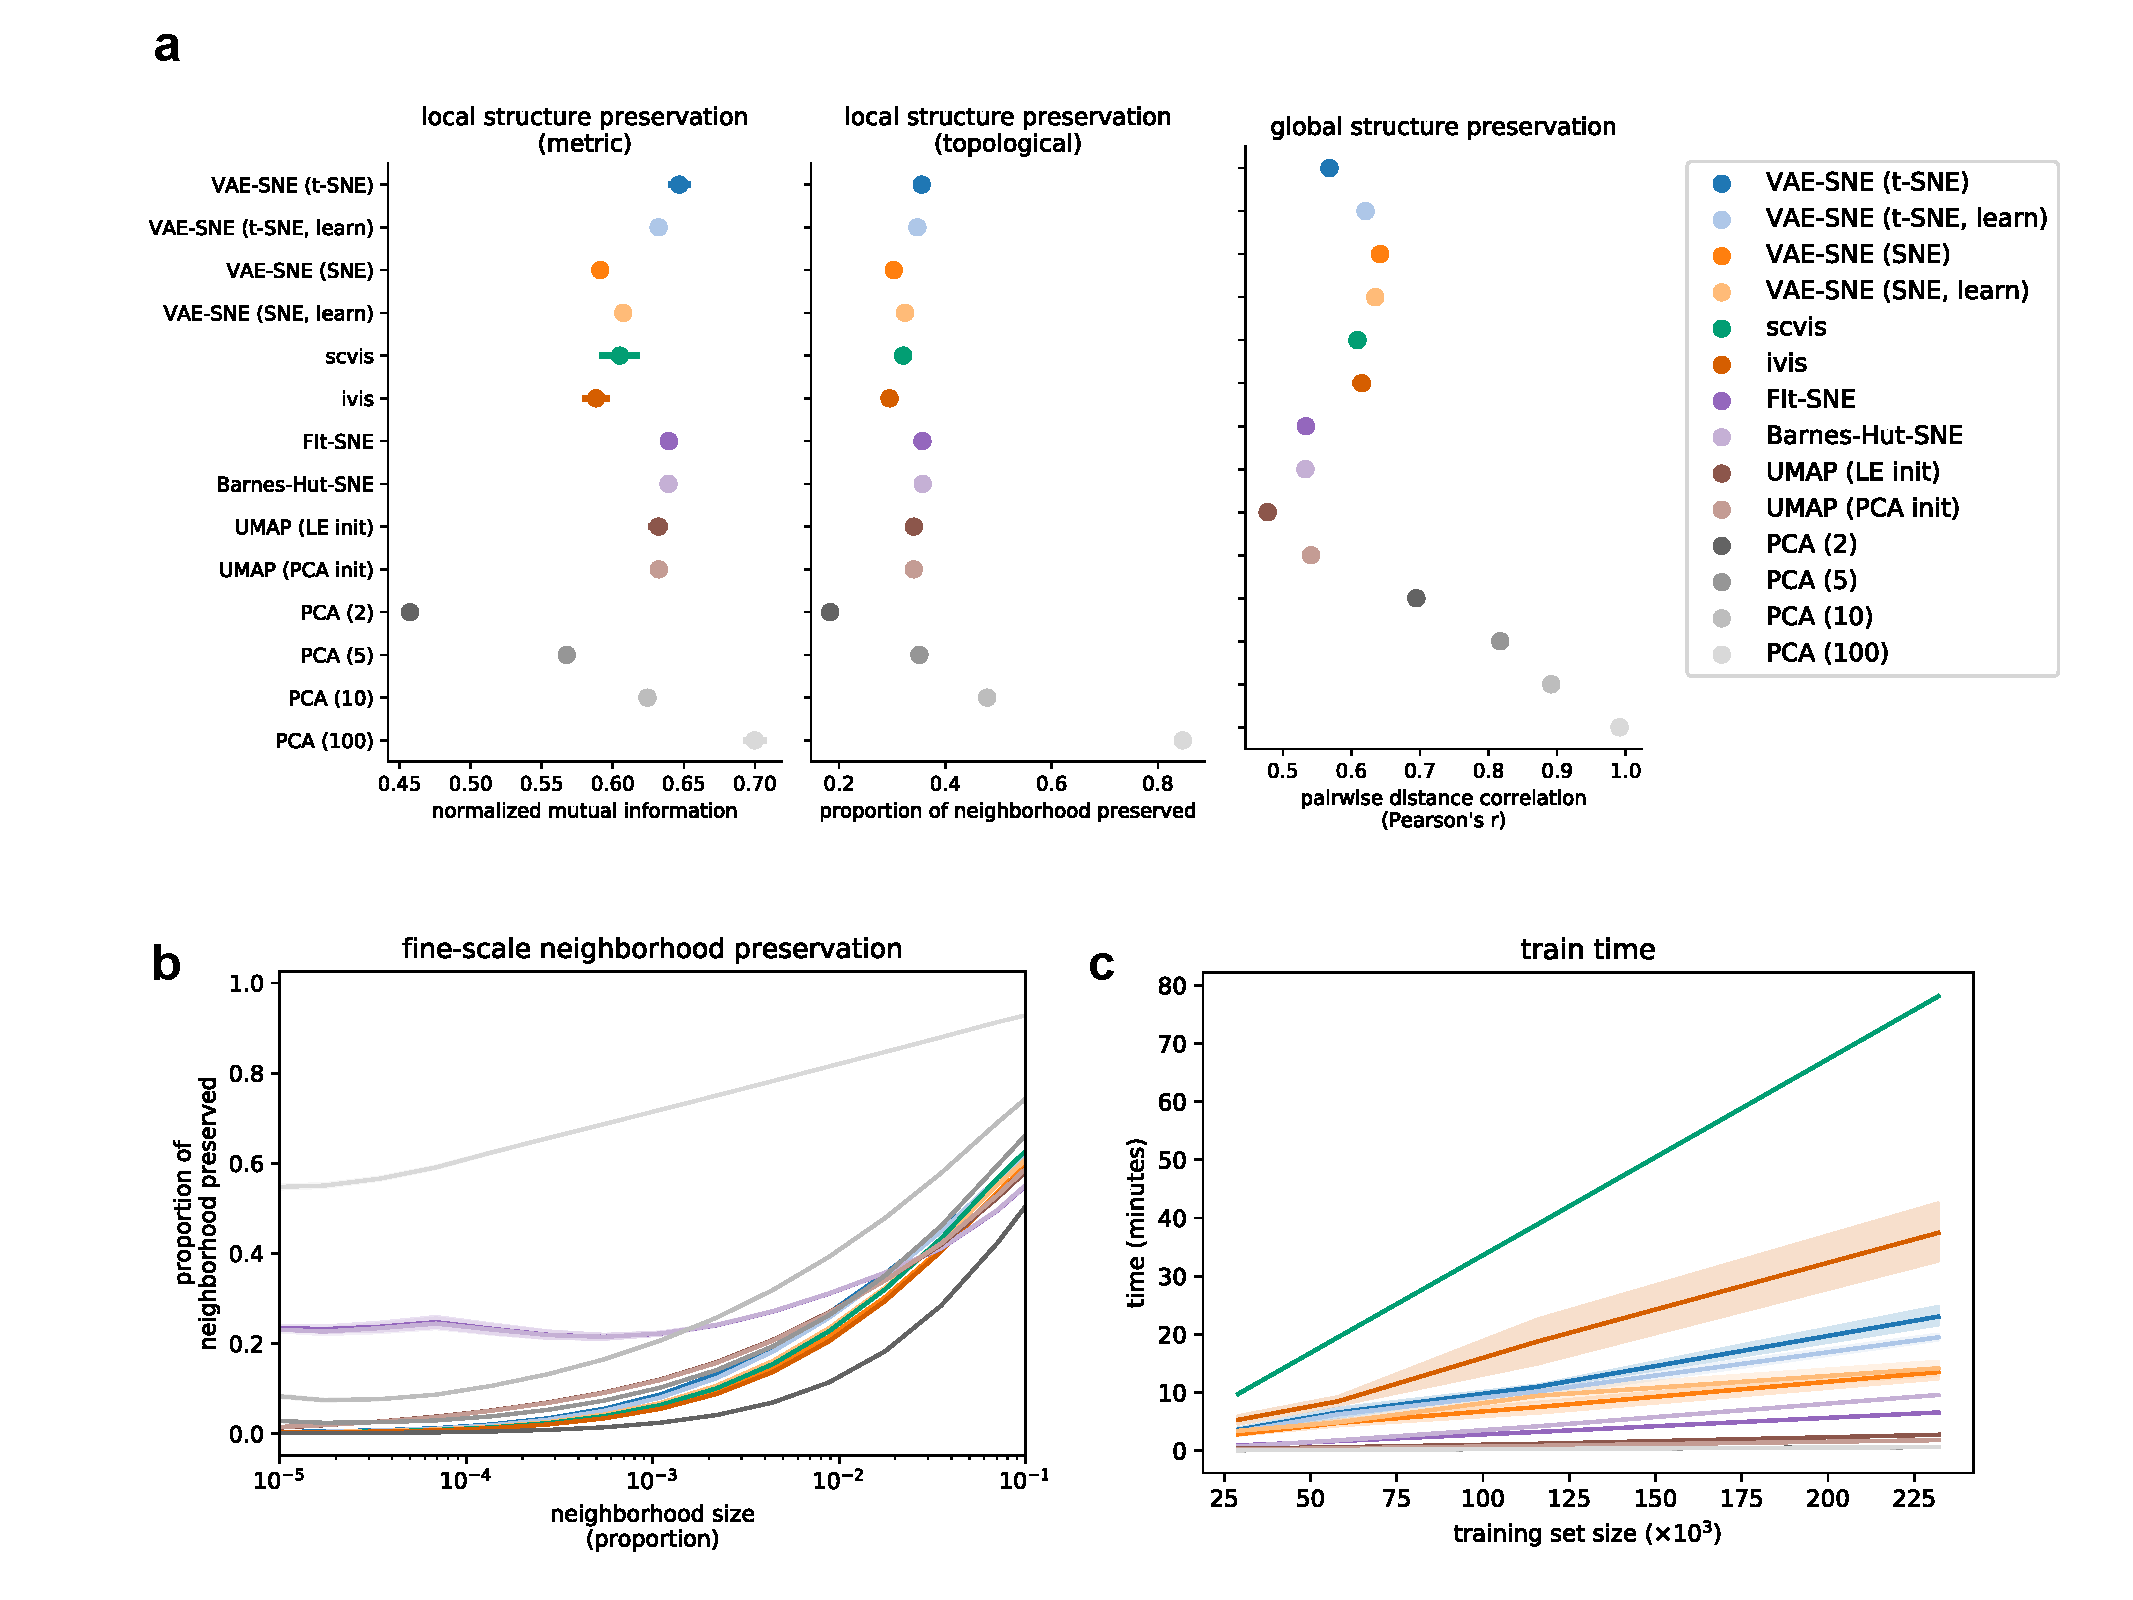
\includegraphics[width=\textwidth]{Graving_IMPRS_Thesis/figures/training_set_figure.pdf}

\caption{  \textbf{Dimension reduction performance for the posture dynamics training set}. Plots show performance comparisons for the posture dynamics dataset \citep{berman2014mapping, berman2016predictability, pereira2019fast} using the training set. \textbf{a}, Mean and 95\% interval of the bootstrap distribution for local and global structure preservation. Results are pooled across all training set sizes (for each metric n = 4 training set sizes $\times$ 5 trials $\times$ 5 replicates = 100 per algorithm). \textbf{b}, Mean and 95\% interval of the bootstrap distribution for fine-scale structure preservation across multiple neighbor sizes (as a proportion of the total embedding size). Results are from the largest training set size only (n = 14 neighborhood sizes $\times$ 5 trials $\times$ 5 replicates = 350 per algorithm). \textbf{c}, Training time for fitting each algorithm across different training set sizes (n = 4 training set sizes $\times$ 5 trials = 20 per algorithm).}

\label{fig:training_set_figure} % \label works only AFTER \caption within figure environment

\end{figure}

\begin{figure}[!htb]
\centering
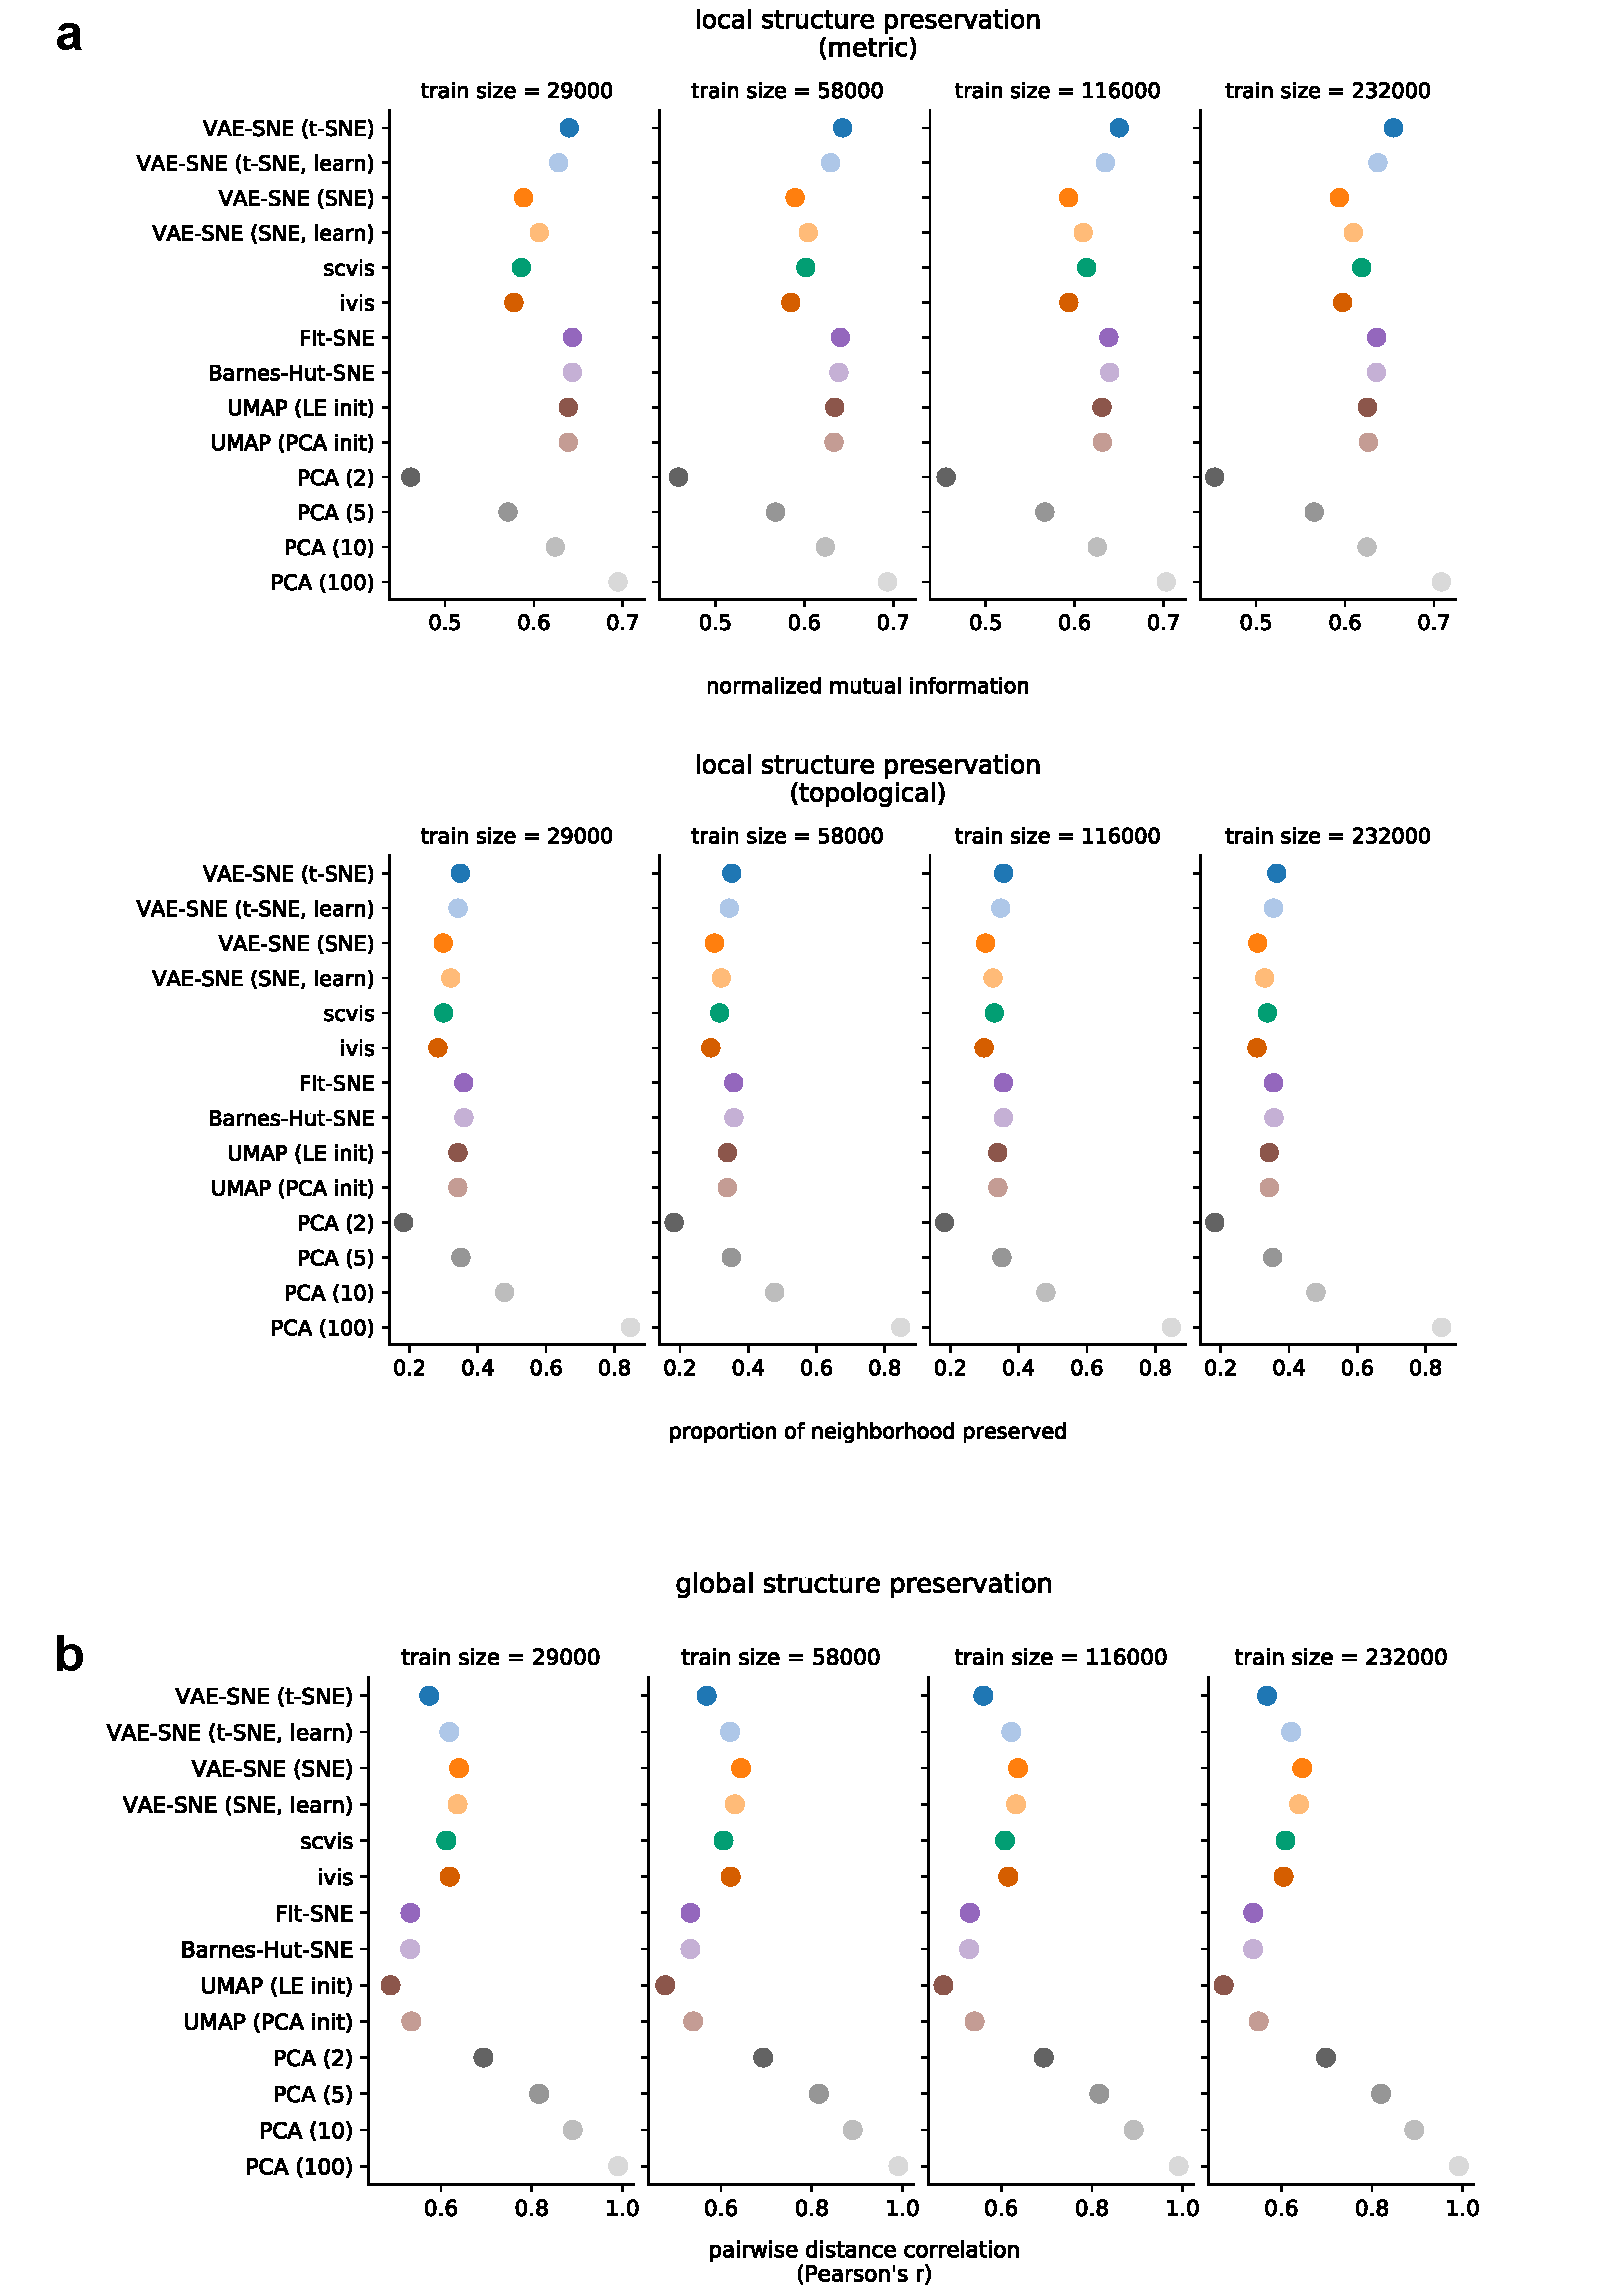
\includegraphics[width=0.9\textwidth]{Graving_IMPRS_Thesis/figures/training_set_appendix_figure.pdf}

\caption{  \textbf{Dimension reduction performance for the posture dynamics training set across training set sizes}. Plots show performance comparisons for the posture dynamics dataset \citep{berman2014mapping, berman2016predictability, pereira2019fast} using training sets of different sizes. \textbf{a-b}, Mean and 95\% interval of the bootstrap distribution for local (\textbf{a}) and global (\textbf{b}) structure preservation. (for each metric n = 5 trials $\times$ 5 replicates = 25 per training set size per algorithm)}

\label{fig:training_set_appendix_figure} % \label works only AFTER \caption within figure environment

\end{figure}



\begin{figure}[!htb]
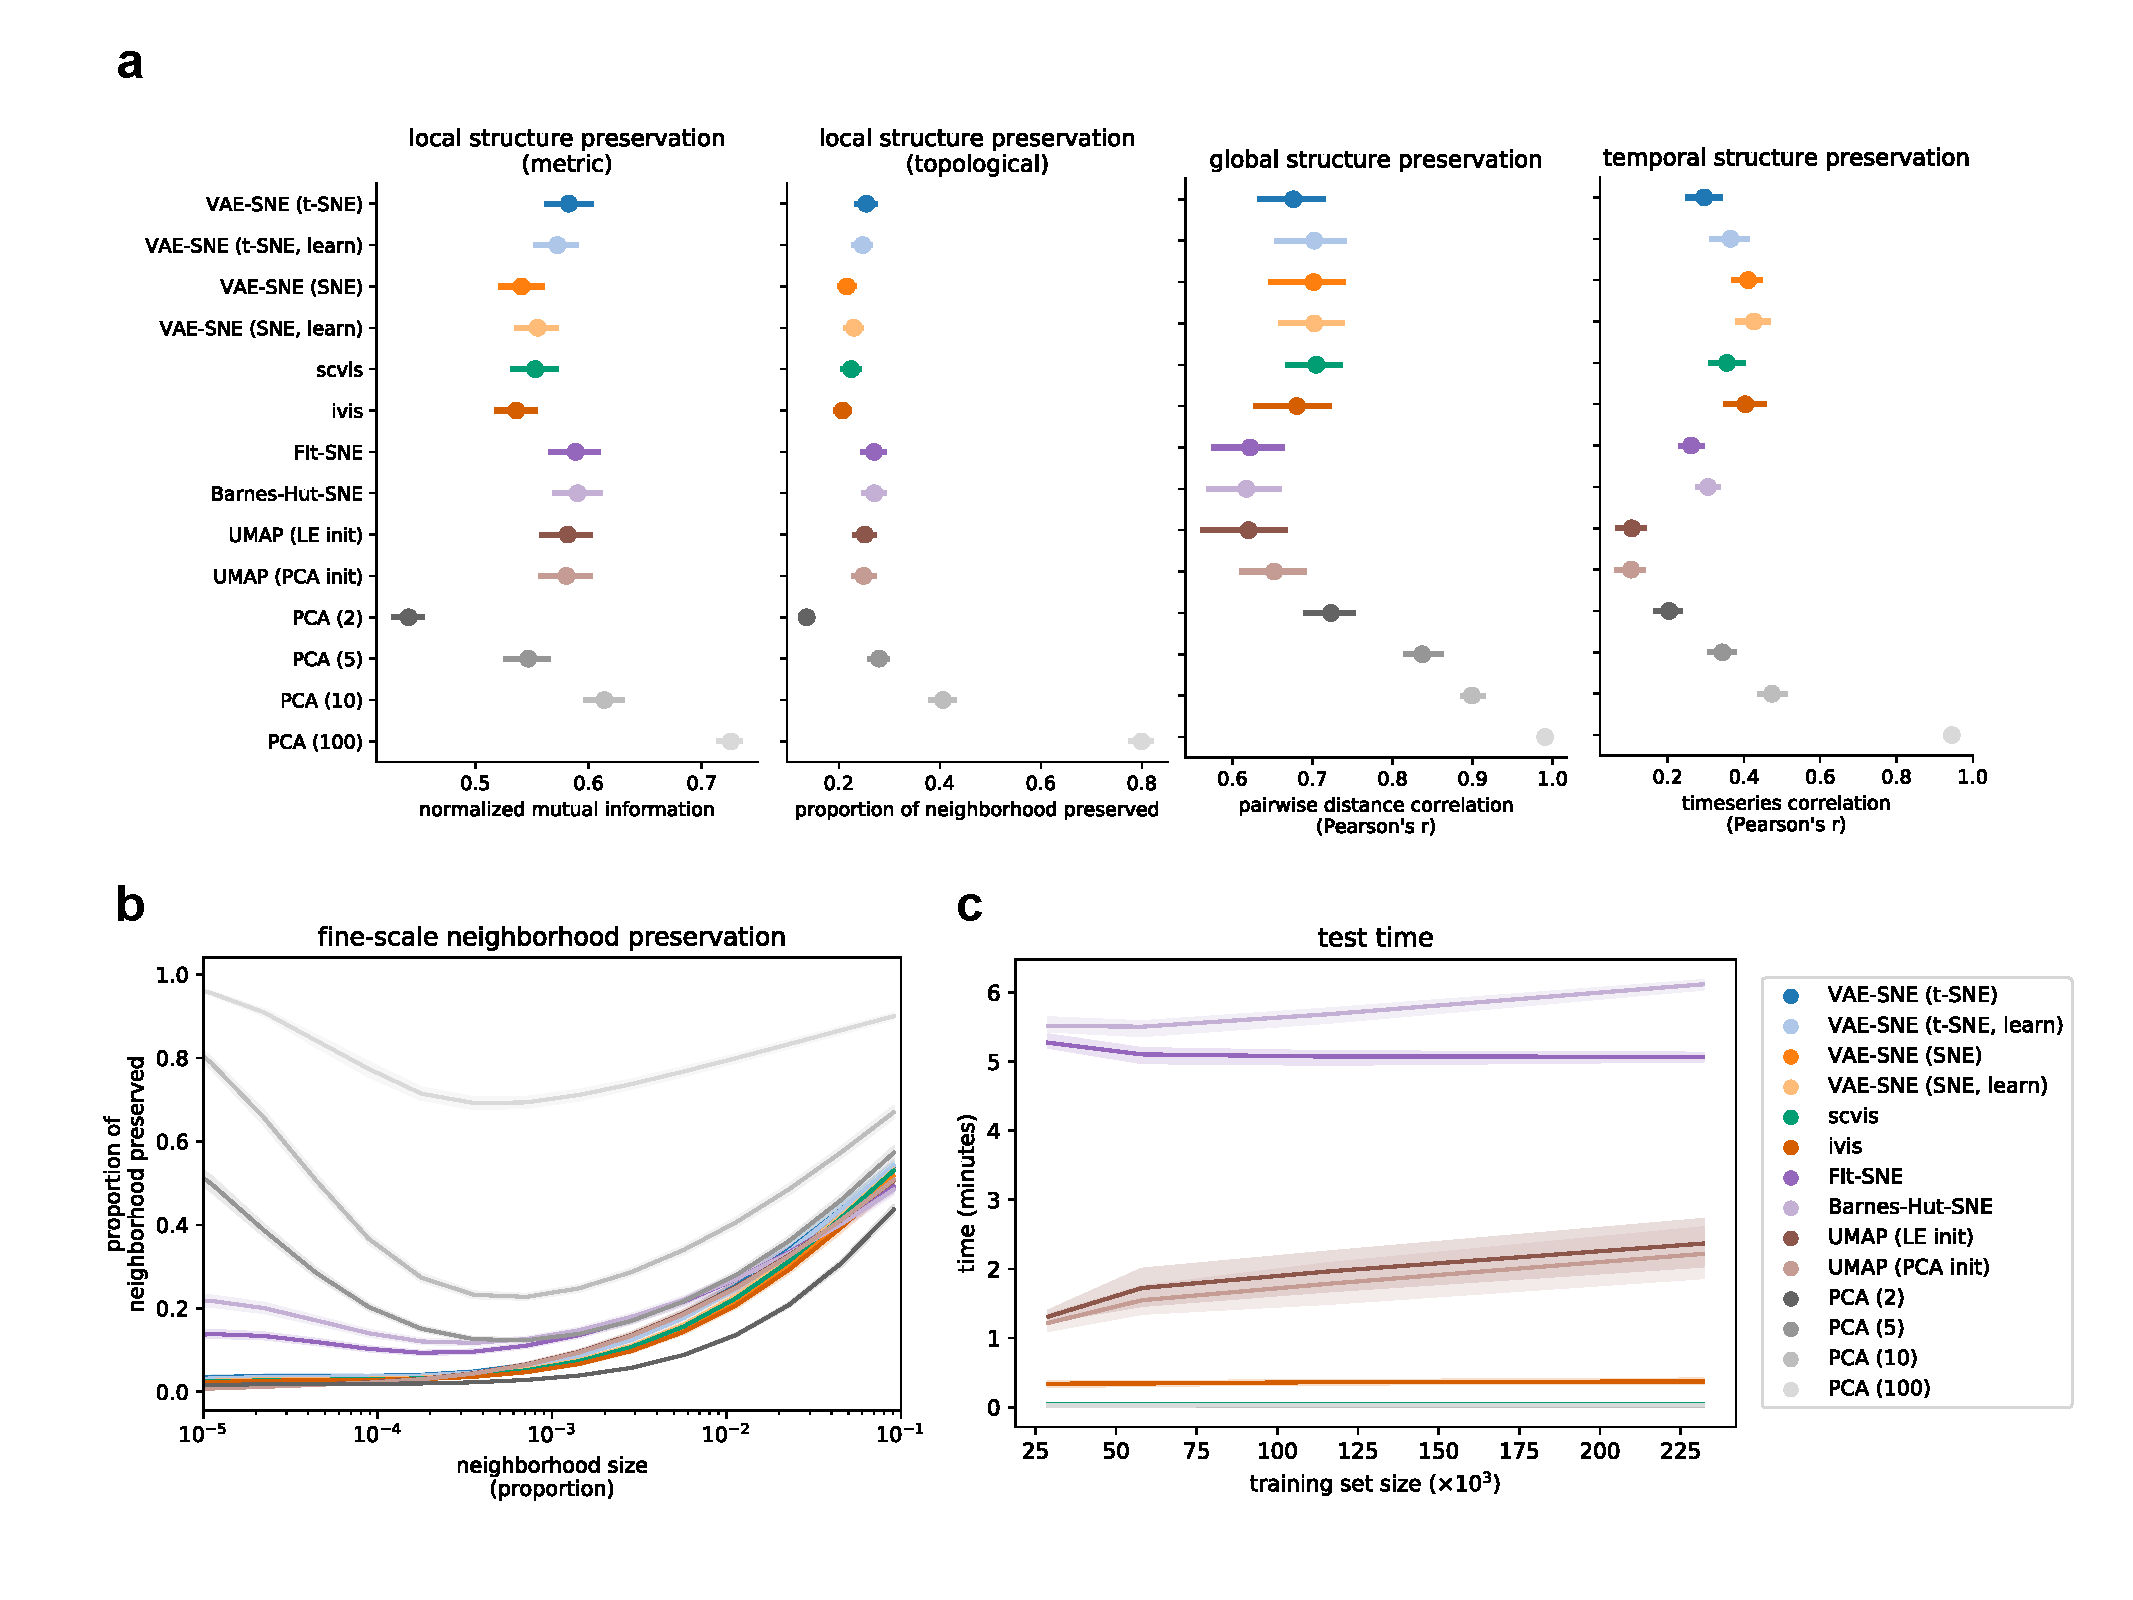
\includegraphics[width=\textwidth]{Graving_IMPRS_Thesis/figures/test_set_figure.pdf}

\caption{  \textbf{Dimension reduction performance for the posture dynamics test set}. Plots show performance comparisons for the posture dynamics dataset \citep{berman2014mapping, berman2016predictability, pereira2019fast} using the test set. \textbf{a}, Mean and 95\% interval of the bootstrap distribution for local, global, and temporal structure preservation. Results are pooled across all training set sizes (for local and global structure n = 4 training set sizes $\times$ 5 trials $\times$ 5 replicates = 100 per algorithm; for temporal structure n = 4 training set sizes $\times$ 5 trials $\times$ 50 subsamples = 1000 per algorithm). \textbf{b}, Mean and 95\% interval of the bootstrap distribution for fine-scale structure preservation across multiple neighbor sizes (as a proportion of the total embedding size). Results are from the largest training set size only (n = 14 neighborhood sizes $\times$ 5 trials $\times$ 5 replicates = 350 per algorithm). \textbf{c}, Elapsed time for embedding the test set with each algorithm across different training set sizes (n = 4 training set sizes $\times$ 5 trials = 20 per algorithm).}

\label{fig:test_set_figure} % \label works only AFTER \caption within figure environment

\end{figure}

\begin{figure}[!htb]
\centering
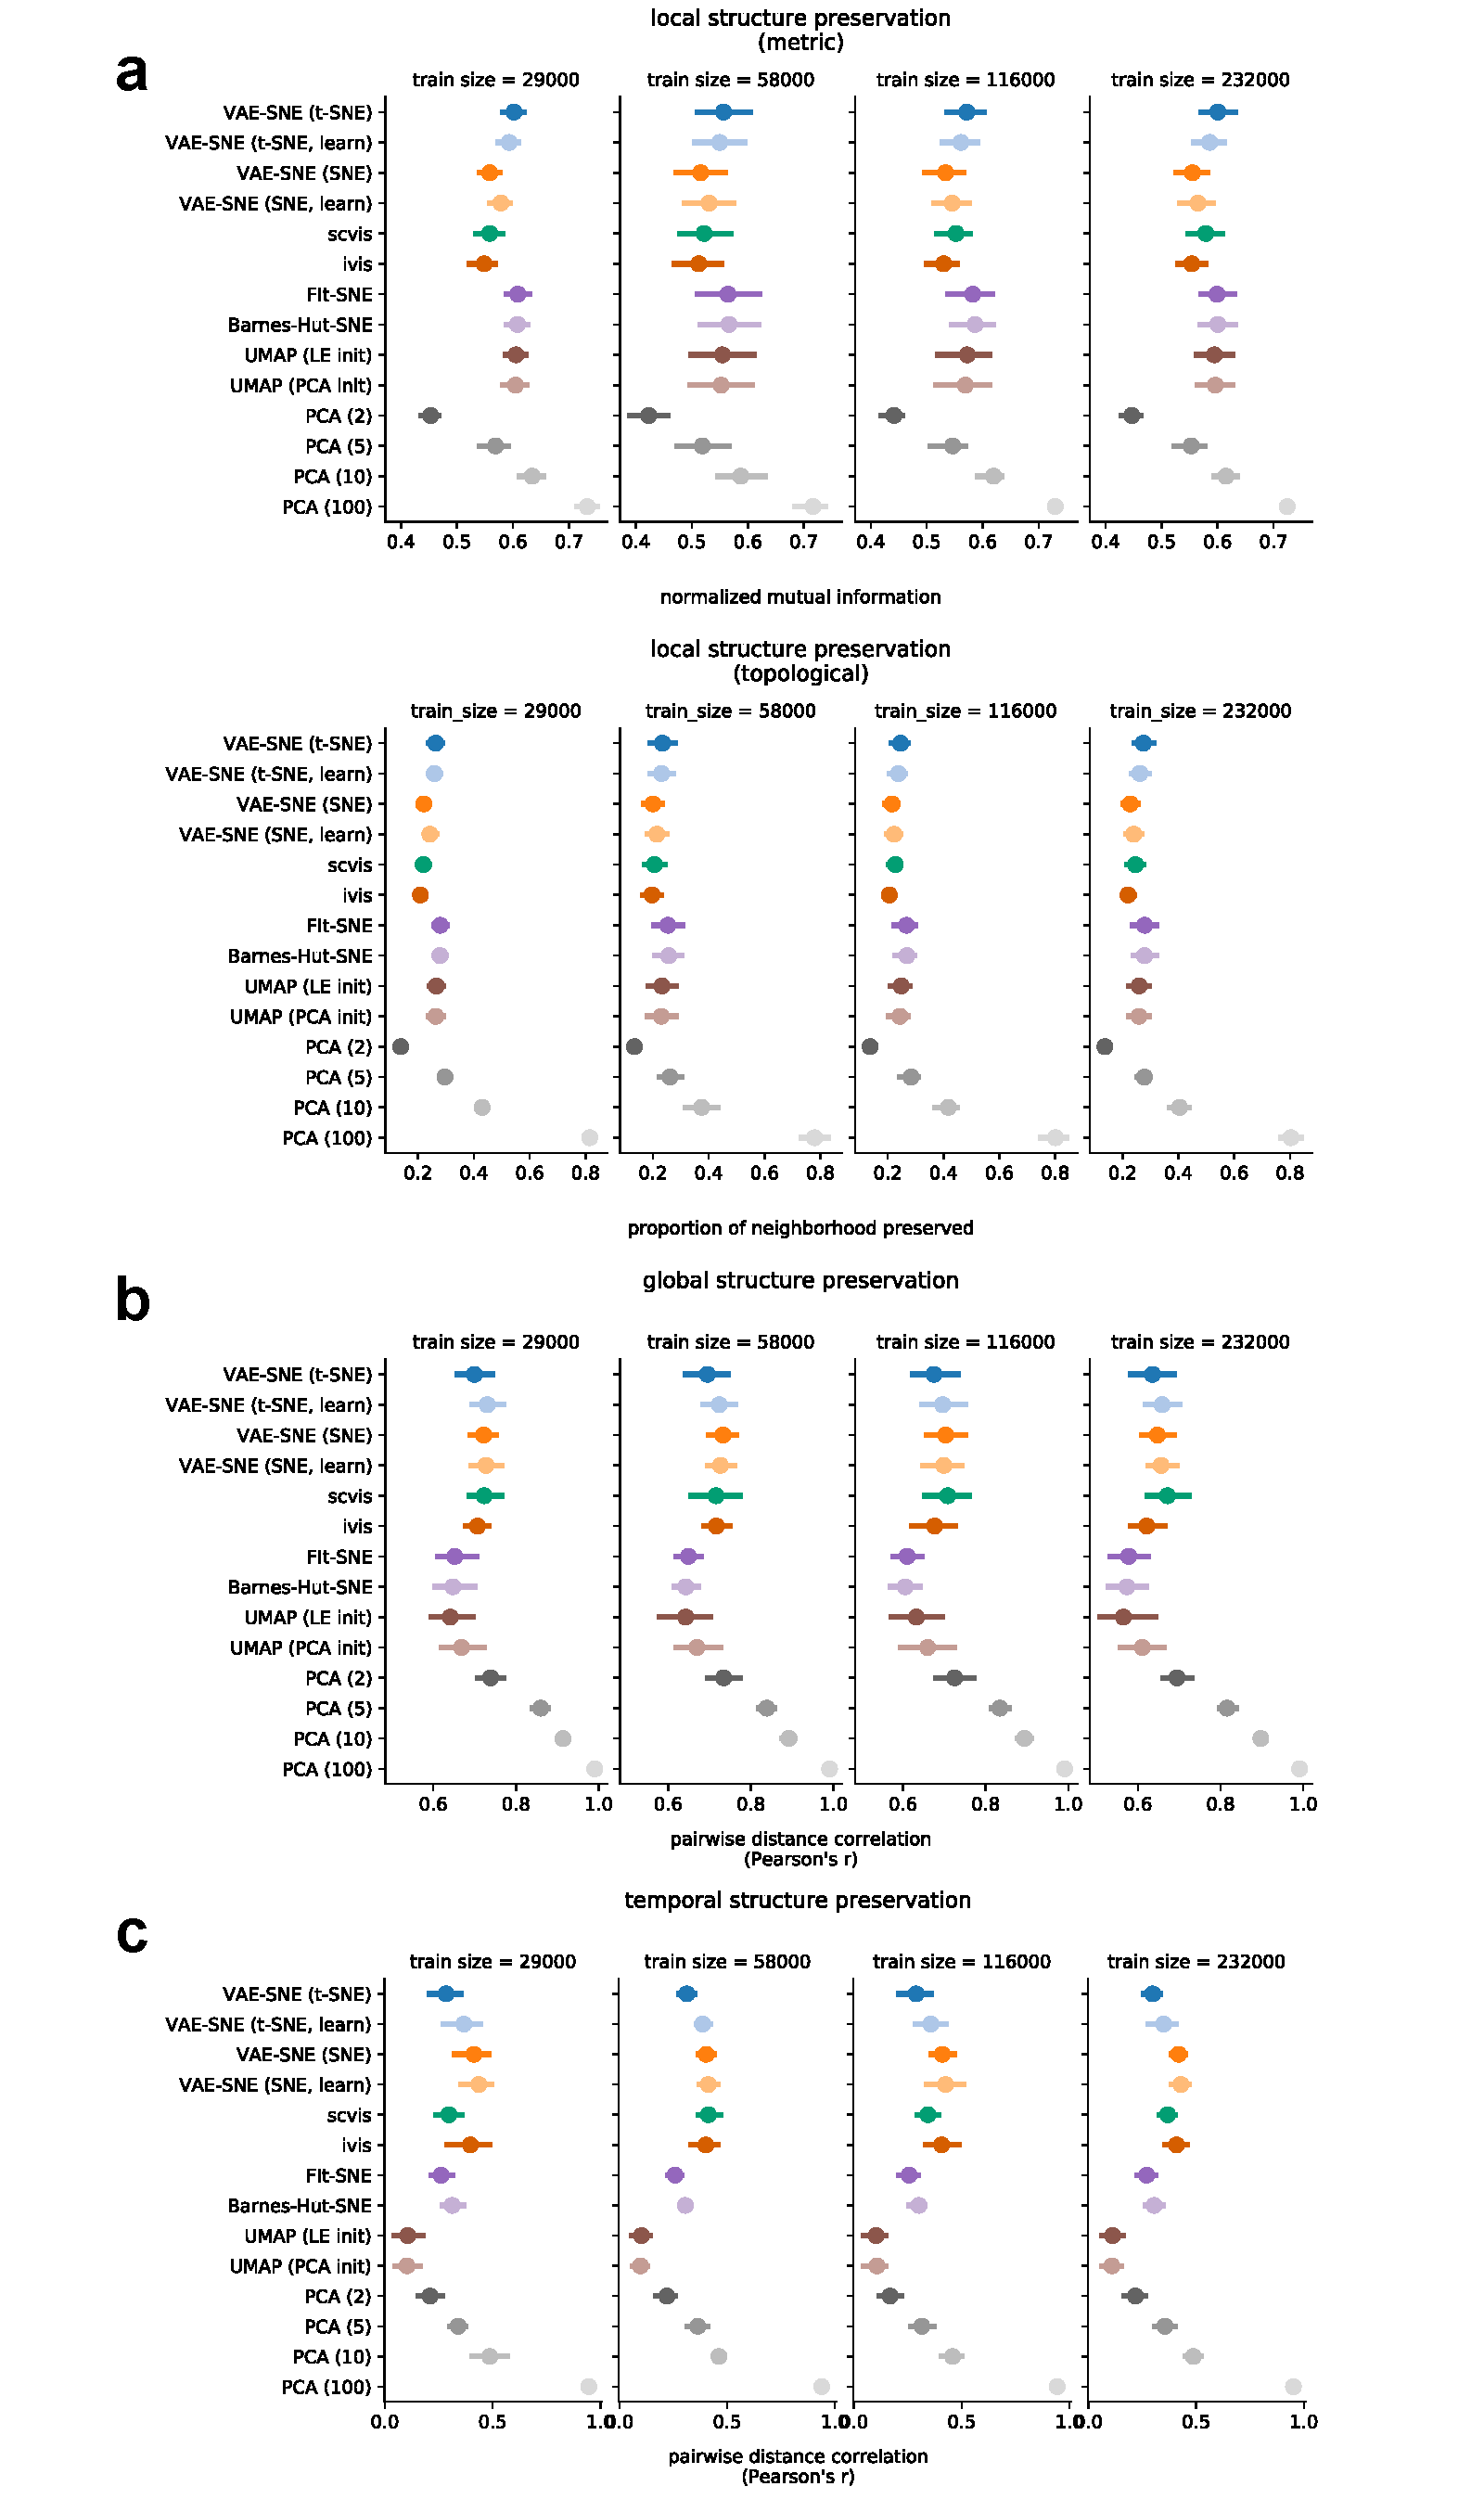
\includegraphics[width=0.75\textwidth]{Graving_IMPRS_Thesis/figures/test_set_appendix_figure.pdf}

\caption{  \textbf{Dimension reduction performance for the posture dynamics test set across training set sizes}. Plots show performance comparisons for the posture dynamics dataset \citep{berman2014mapping, berman2016predictability, pereira2019fast} using training sets of different sizes. \textbf{a-c}, Mean and 95\% interval of the bootstrap distribution for local (\textbf{a}), global (\textbf{b}), and temporal (\textbf{c}) structure preservation (for local and global structure n = 5 trials $\times$ 5 replicates = 25 per algorithm for each training set size; for temporal structure n = 5 trials $\times$ 50 subsamples = 250 per algorithm for each training set size).}

\label{fig:test_set_appendix_figure} % \label works only AFTER \caption within figure environment

\end{figure}


\begin{figure}[!htb]
\begin{center}
    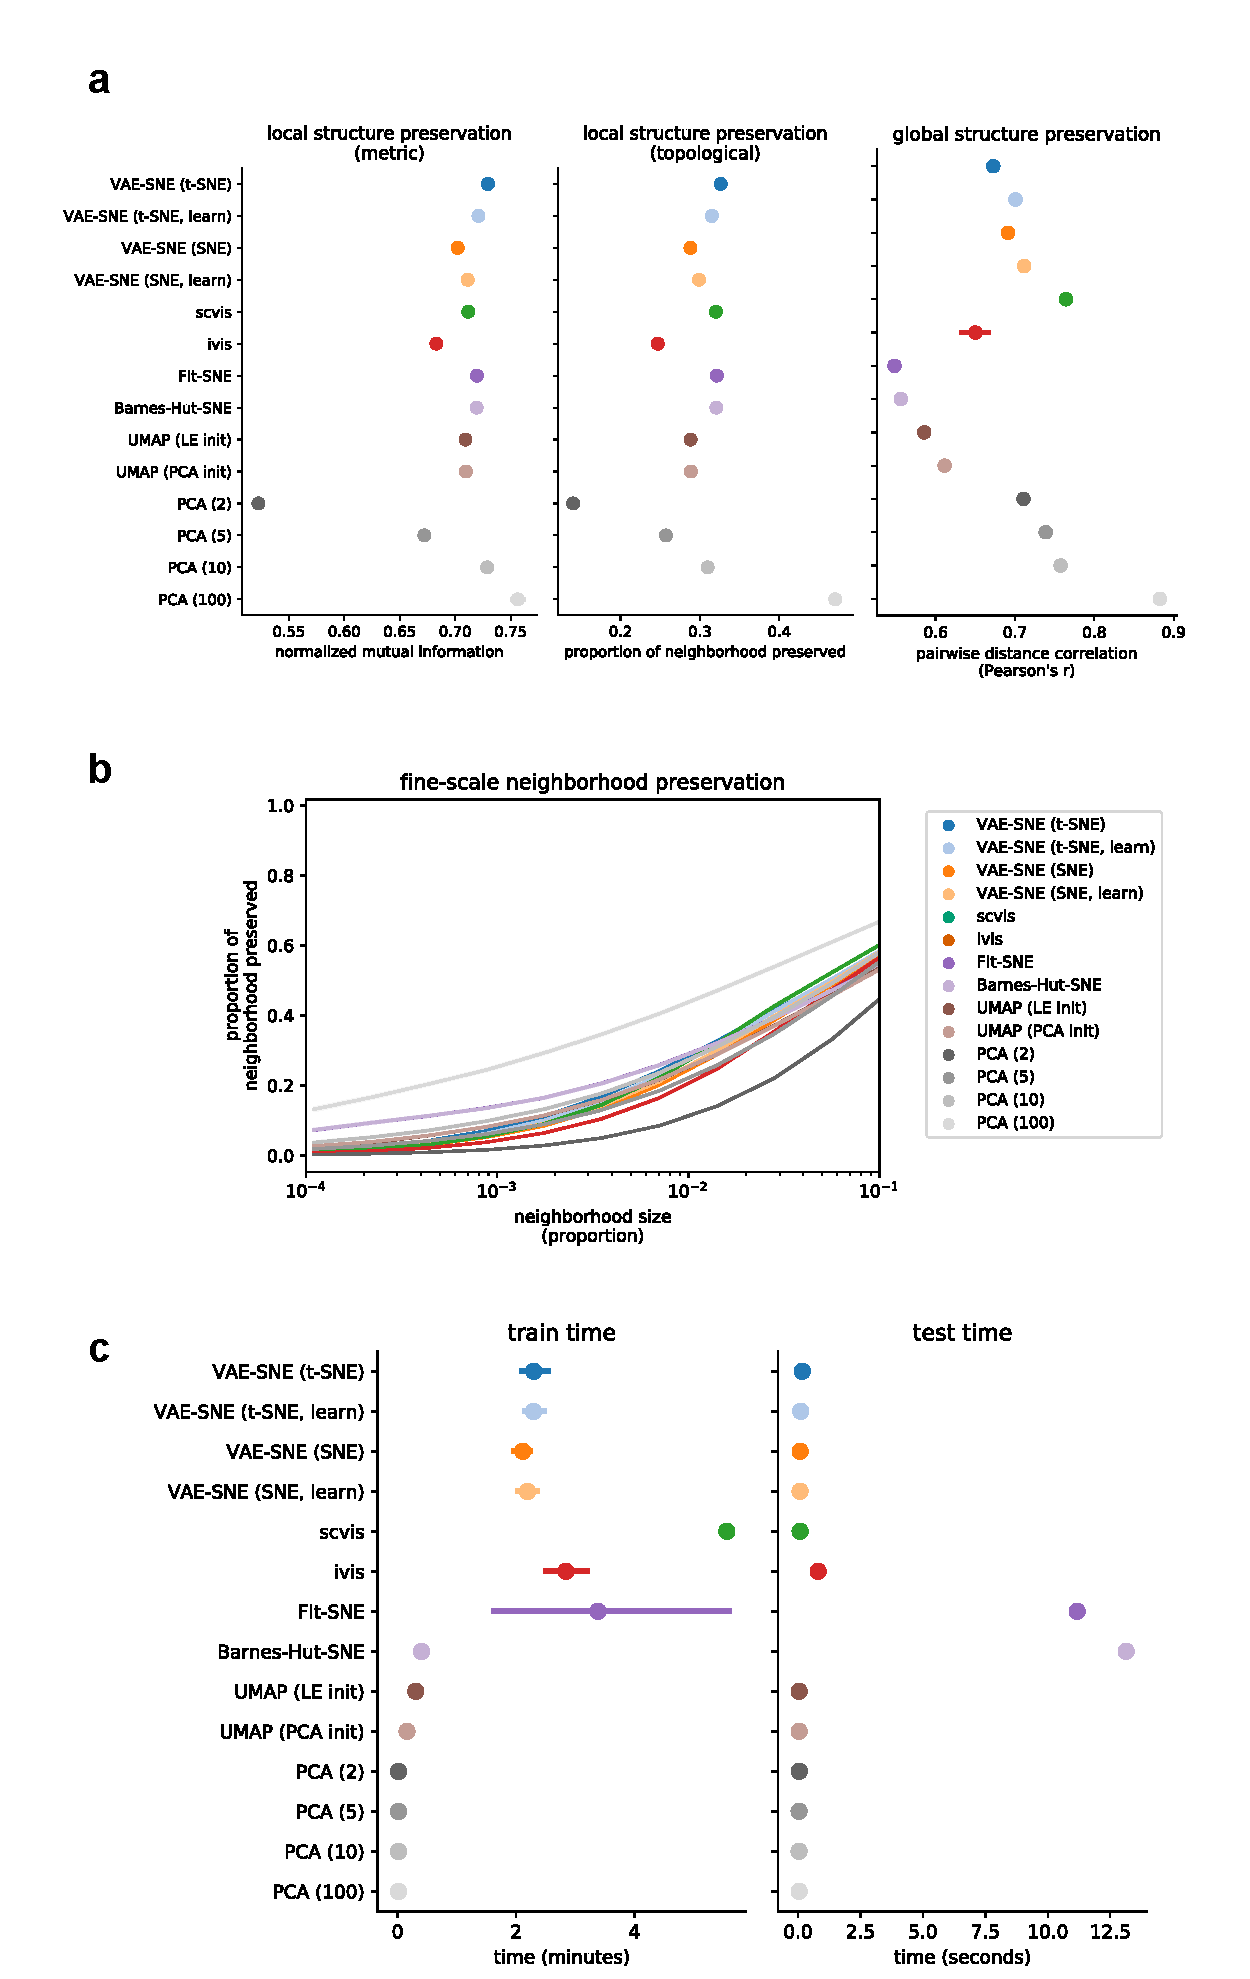
\includegraphics[width=0.7\textwidth]{Graving_IMPRS_Thesis/figures/rna_velocity_figure.pdf}
\end{center}

\caption{  \textbf{Dimension reduction performance for the single-cell RNA-seq dataset}. Plots show performance comparisons for the single-cell RNA-seq dataset from \cite{la2018rna} using the entire dataset. \textbf{a}, Mean and 95\% interval of the bootstrap distribution for local and global structure preservation (for each metric n = 5 trials $\times$ 5 replicates = 25 per algorithm). \textbf{b}, Mean and 95\% interval of the bootstrap distribution for fine-scale structure preservation across multiple neighbor sizes (as a proportion of the total embedding size; n = 14 neighborhood sizes $\times$ 5 trials $\times$ 5 replicates = 350 per algorithm). \textbf{c}, Elapsed time for embedding the training set and re-embedding the training set as a ``test" set with each algorithm (for each metric n = 5 trials $\times$ 5 replicates = 25 per algorithm).}

\label{fig:rna_velocity_figure} % \label works only AFTER \caption within figure environment

\end{figure}

\begin{figure}[!htb]
\begin{center}
    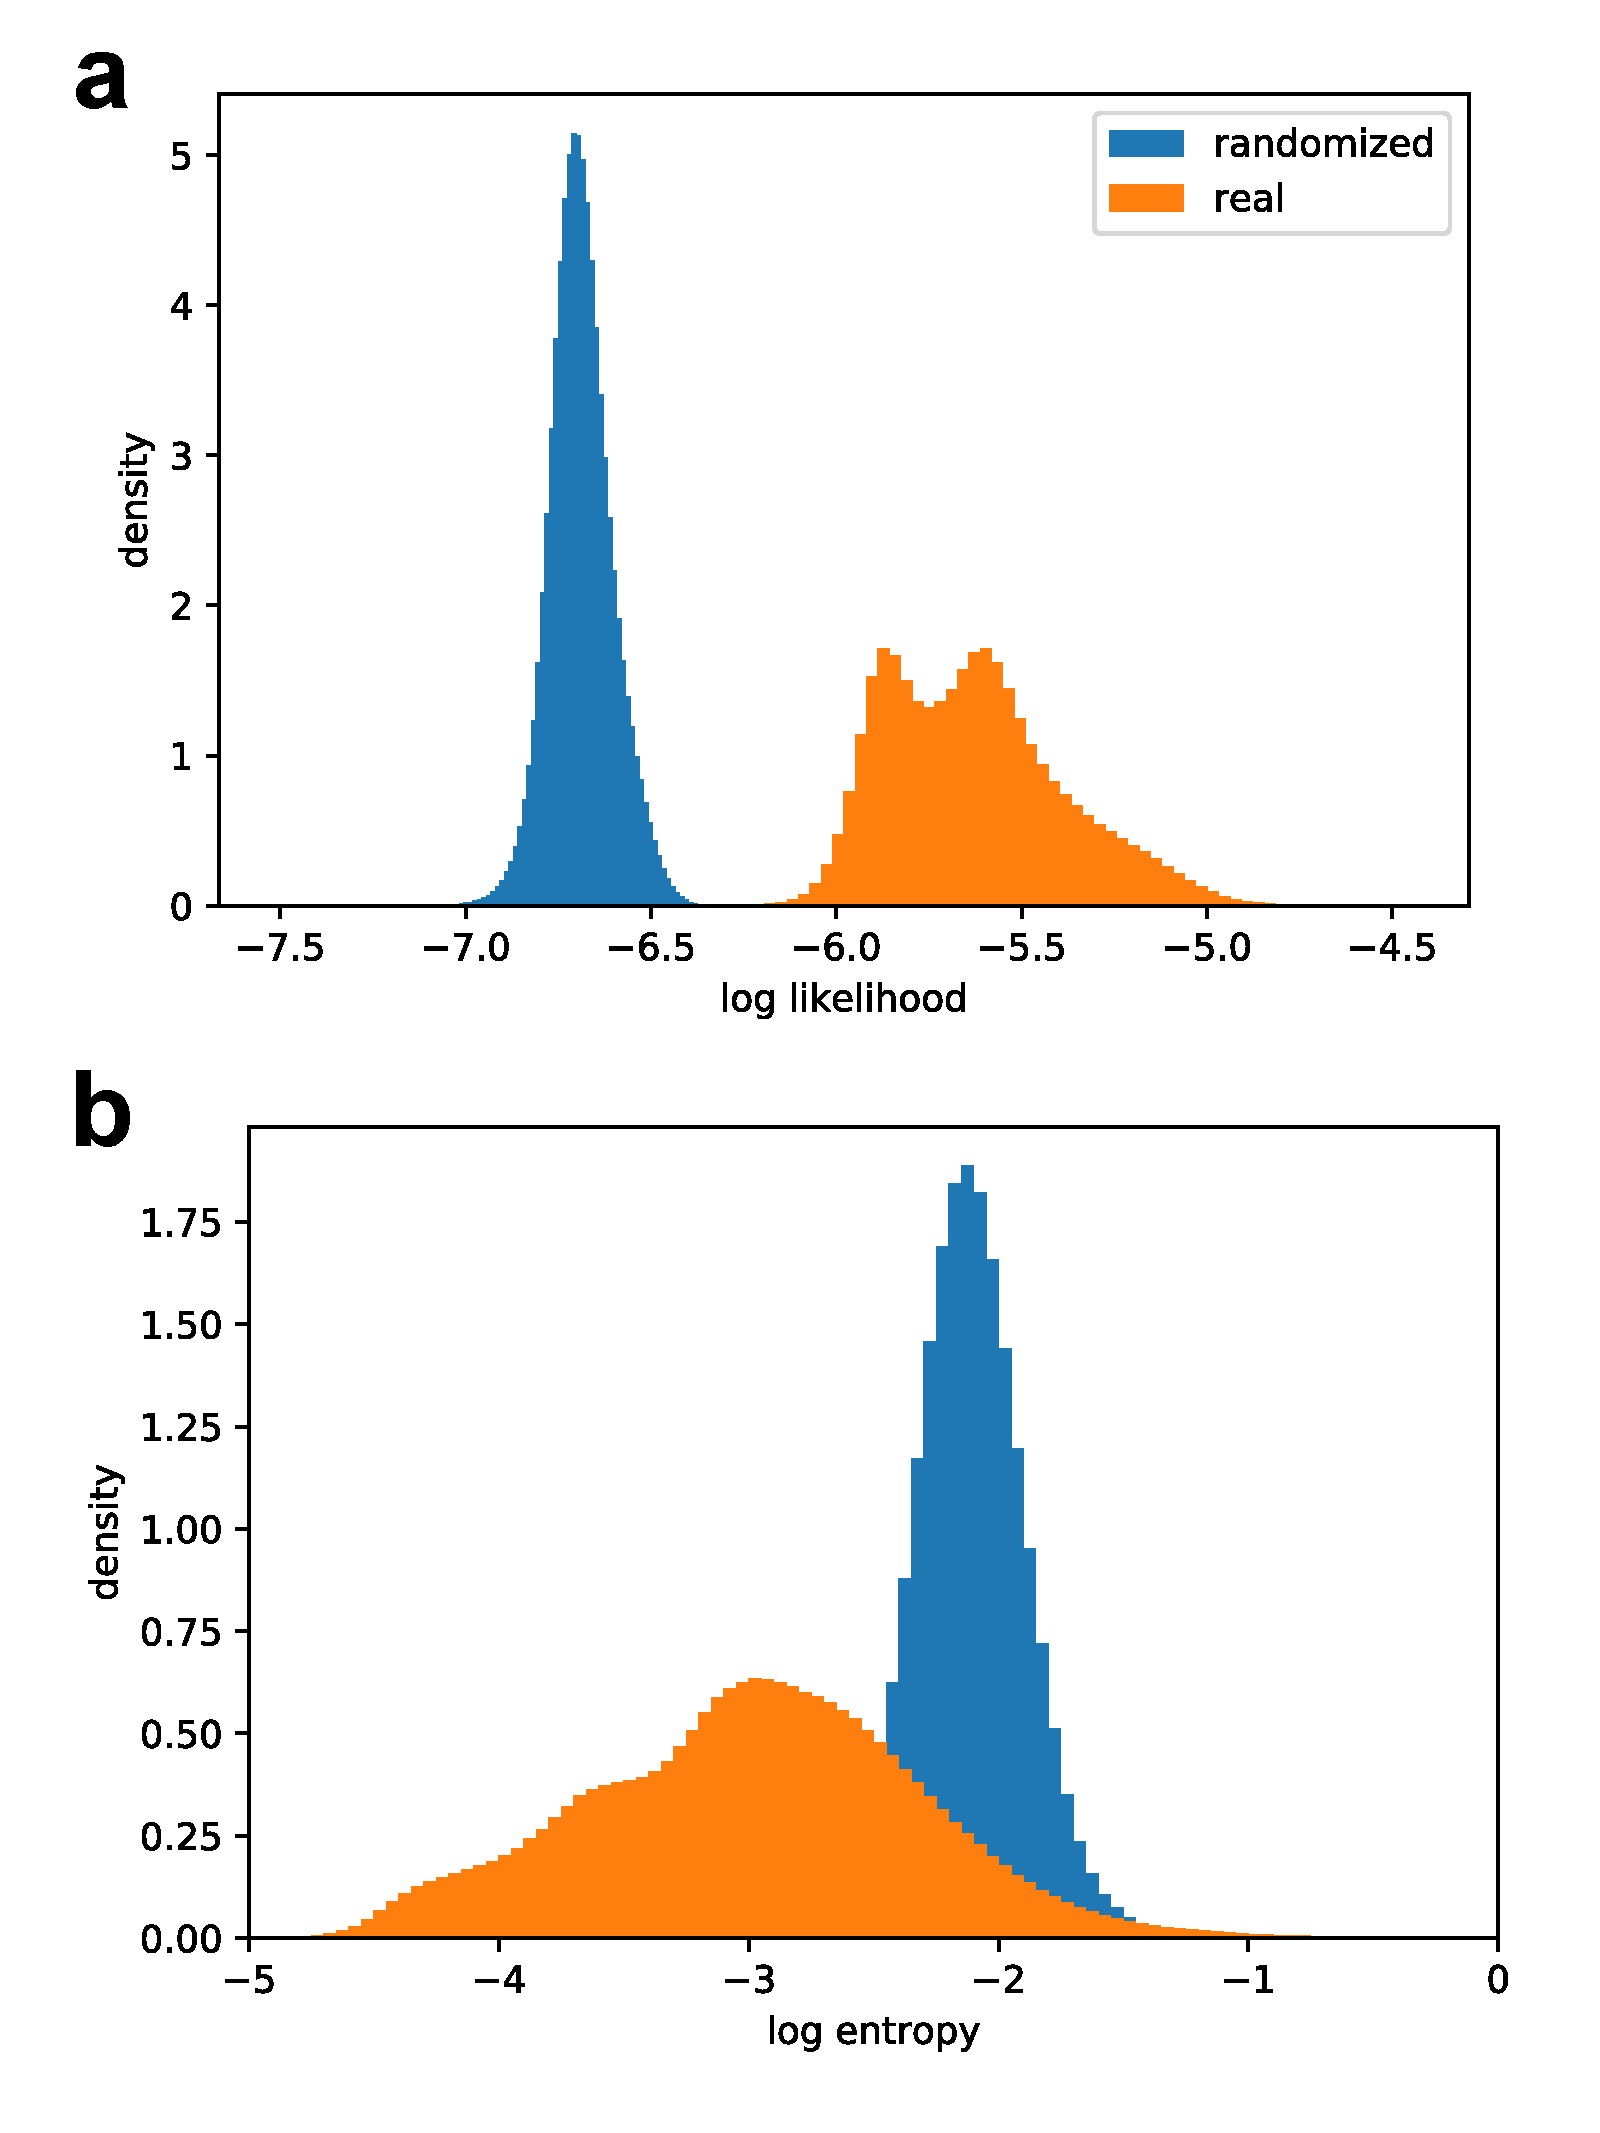
\includegraphics[width=0.5\textwidth]{Graving_IMPRS_Thesis/figures/likelihood_entropy_figure.pdf}
\end{center}

\caption{  \textbf{Likelihood and entropy distributions}. \textbf{a}, Histograms of the log likelihood scores from the decoder (Eq. \ref{eq:elbo}; distortion) for real and randomized data (n = 232,000 for each distribution). \textbf{b}, Histograms of the log entropy from the approximate posterior (Eq. \ref{eq:approx}) for real and randomized data (n = 232,000 for each distribution).}

\label{fig:likelihood_entropy_figure} % \label works only AFTER \caption within figure environment

\end{figure}

\begin{figure}[!htb]
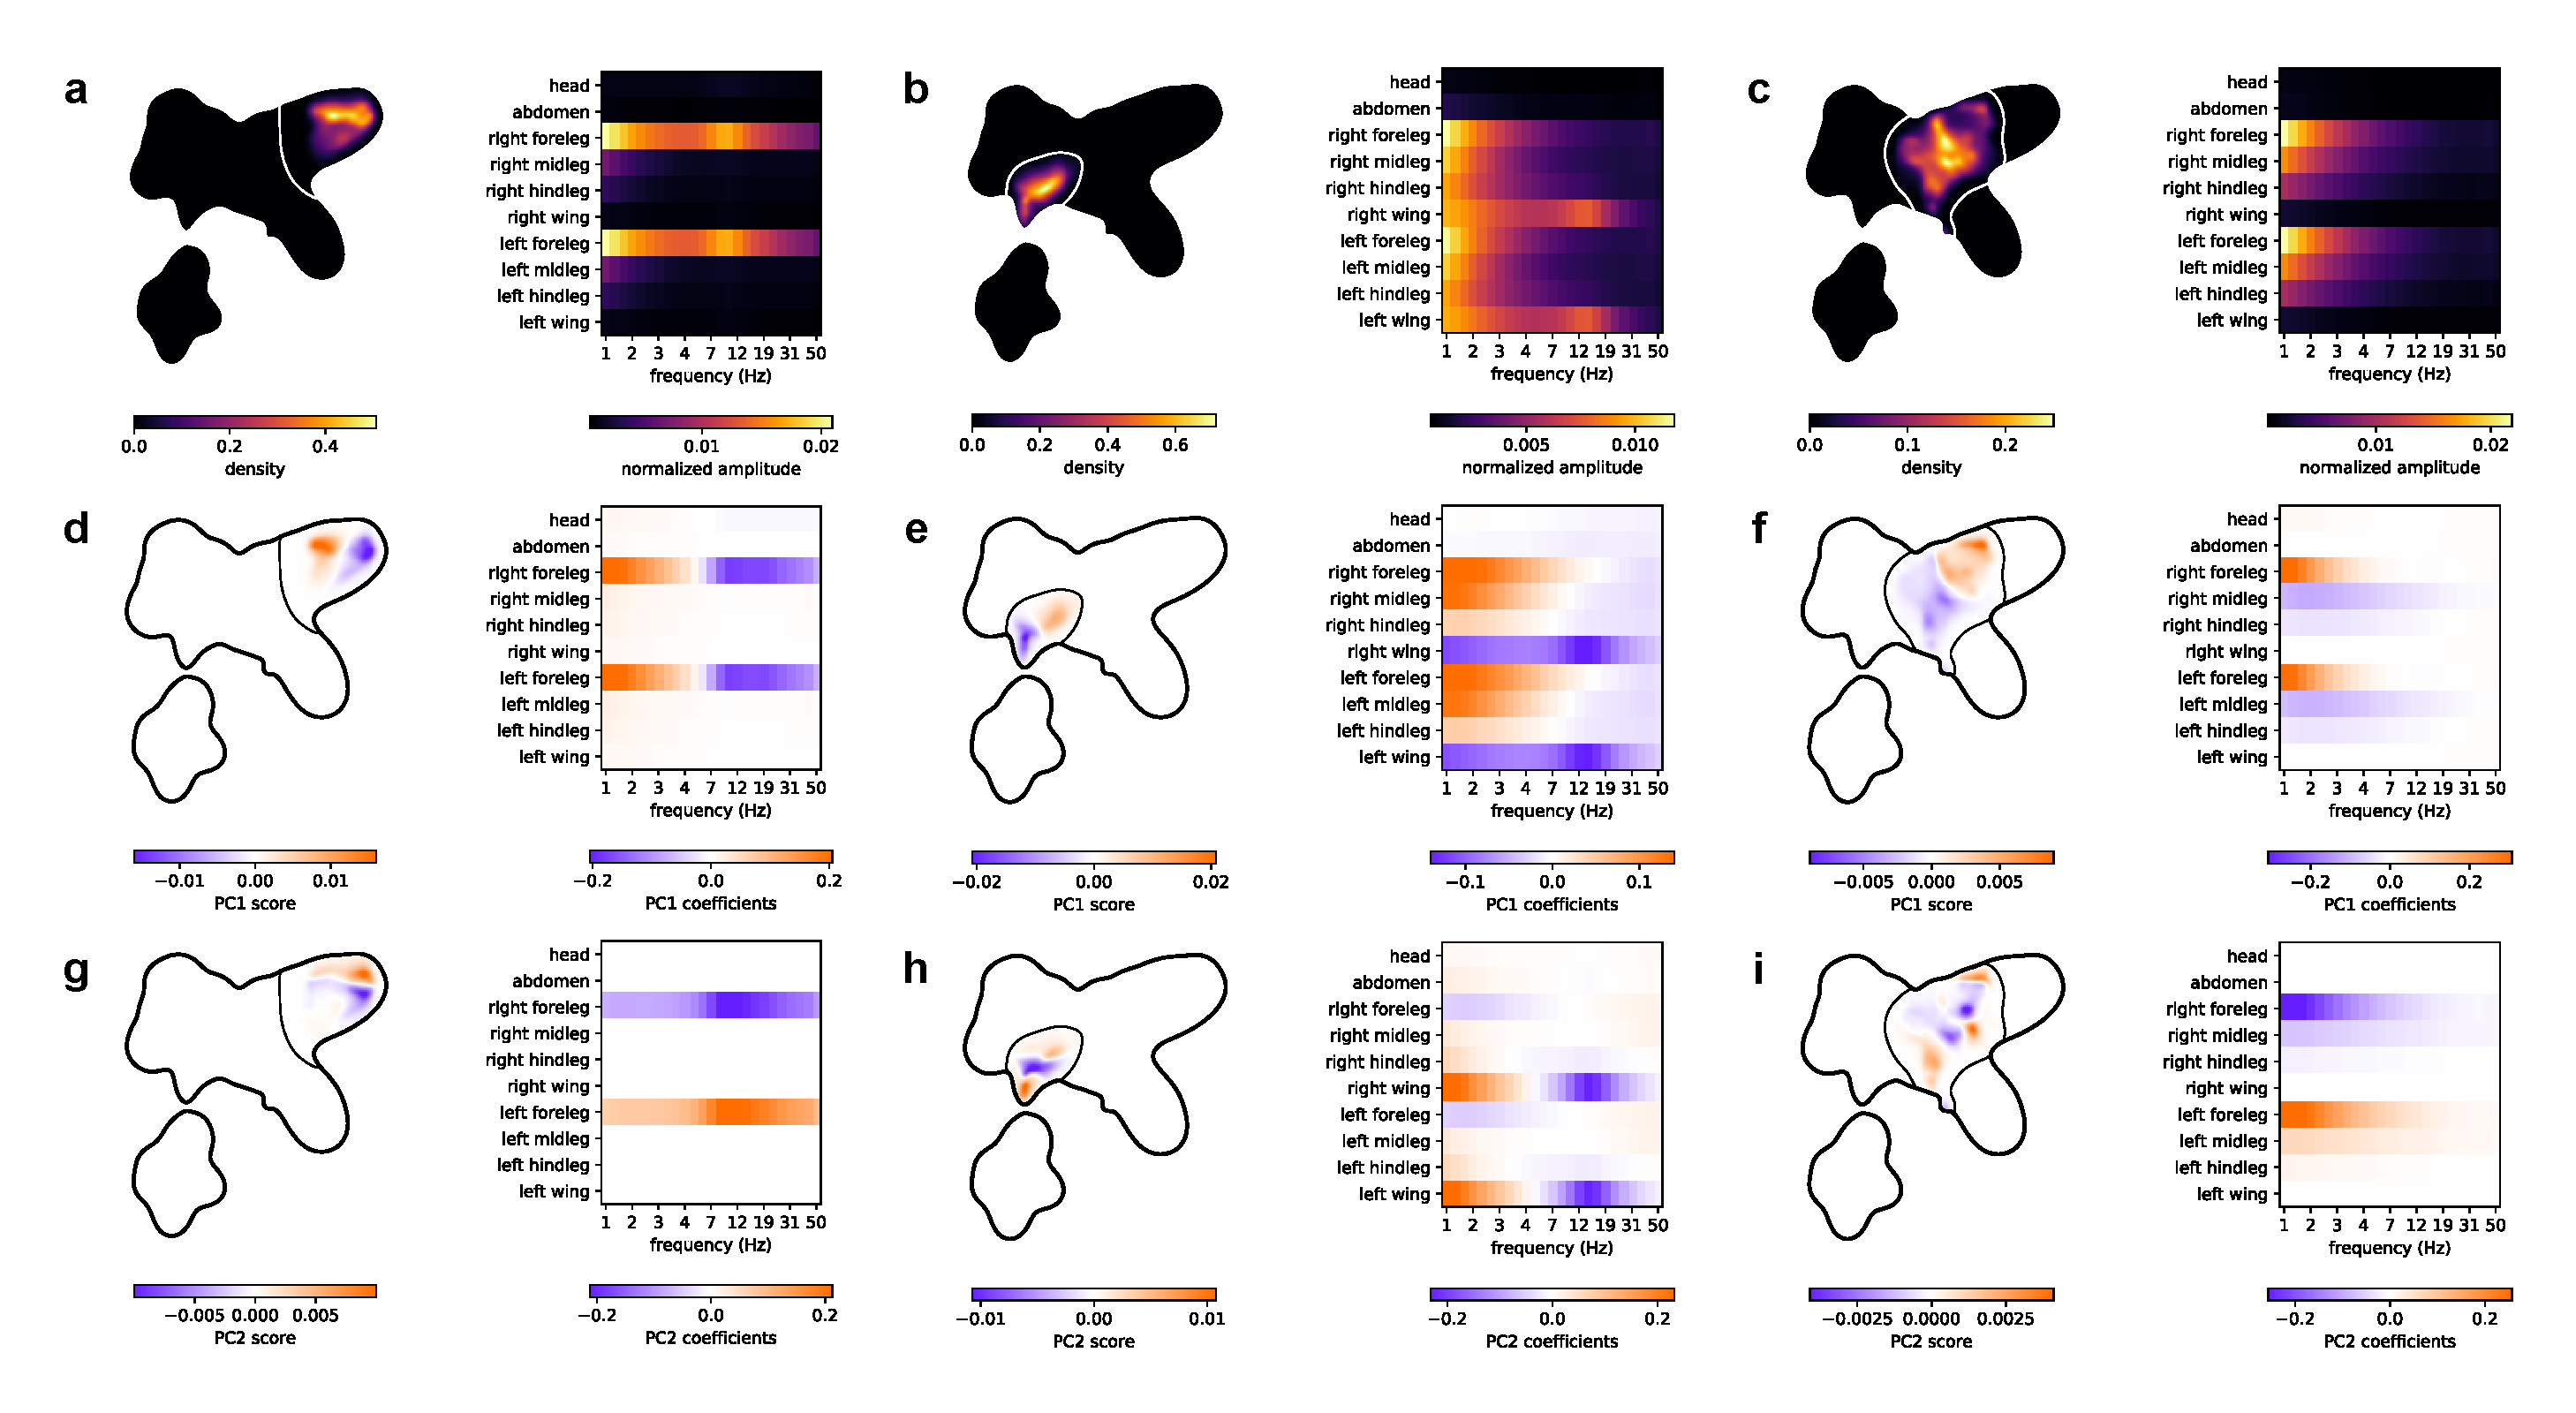
\includegraphics[width=1.0\textwidth]{Graving_IMPRS_Thesis/figures/cluster_appendix.pdf}

\caption{  \textbf{High-level behavioral clusters.} Visualizations describing the manually-grouped high-level clusters for anterior grooming (\textbf{a},\textbf{e},\textbf{g}), wing movements (\textbf{b},\textbf{e},\textbf{h}) and small/slow leg movements (\textbf{c},\textbf{f},\textbf{i}). \textbf{a-c}, The 2-D posterior probability density for each cluster (left), where contours are the largest 90\% probability density contour for each cluster distribution, and the mean spectrogram for each cluster (right). \textbf{d}-\textbf{i}, The principal component scores of the spectrograms assigned to each cluster visualized within the 2-D embedding (left) and the eigenvector coefficients describing the linear contribution of each spectrogram feature (right) for the principal component score.}

\label{fig:cluster_appendix_figure}

\end{figure}

\begin{figure}[!htb]
\centering
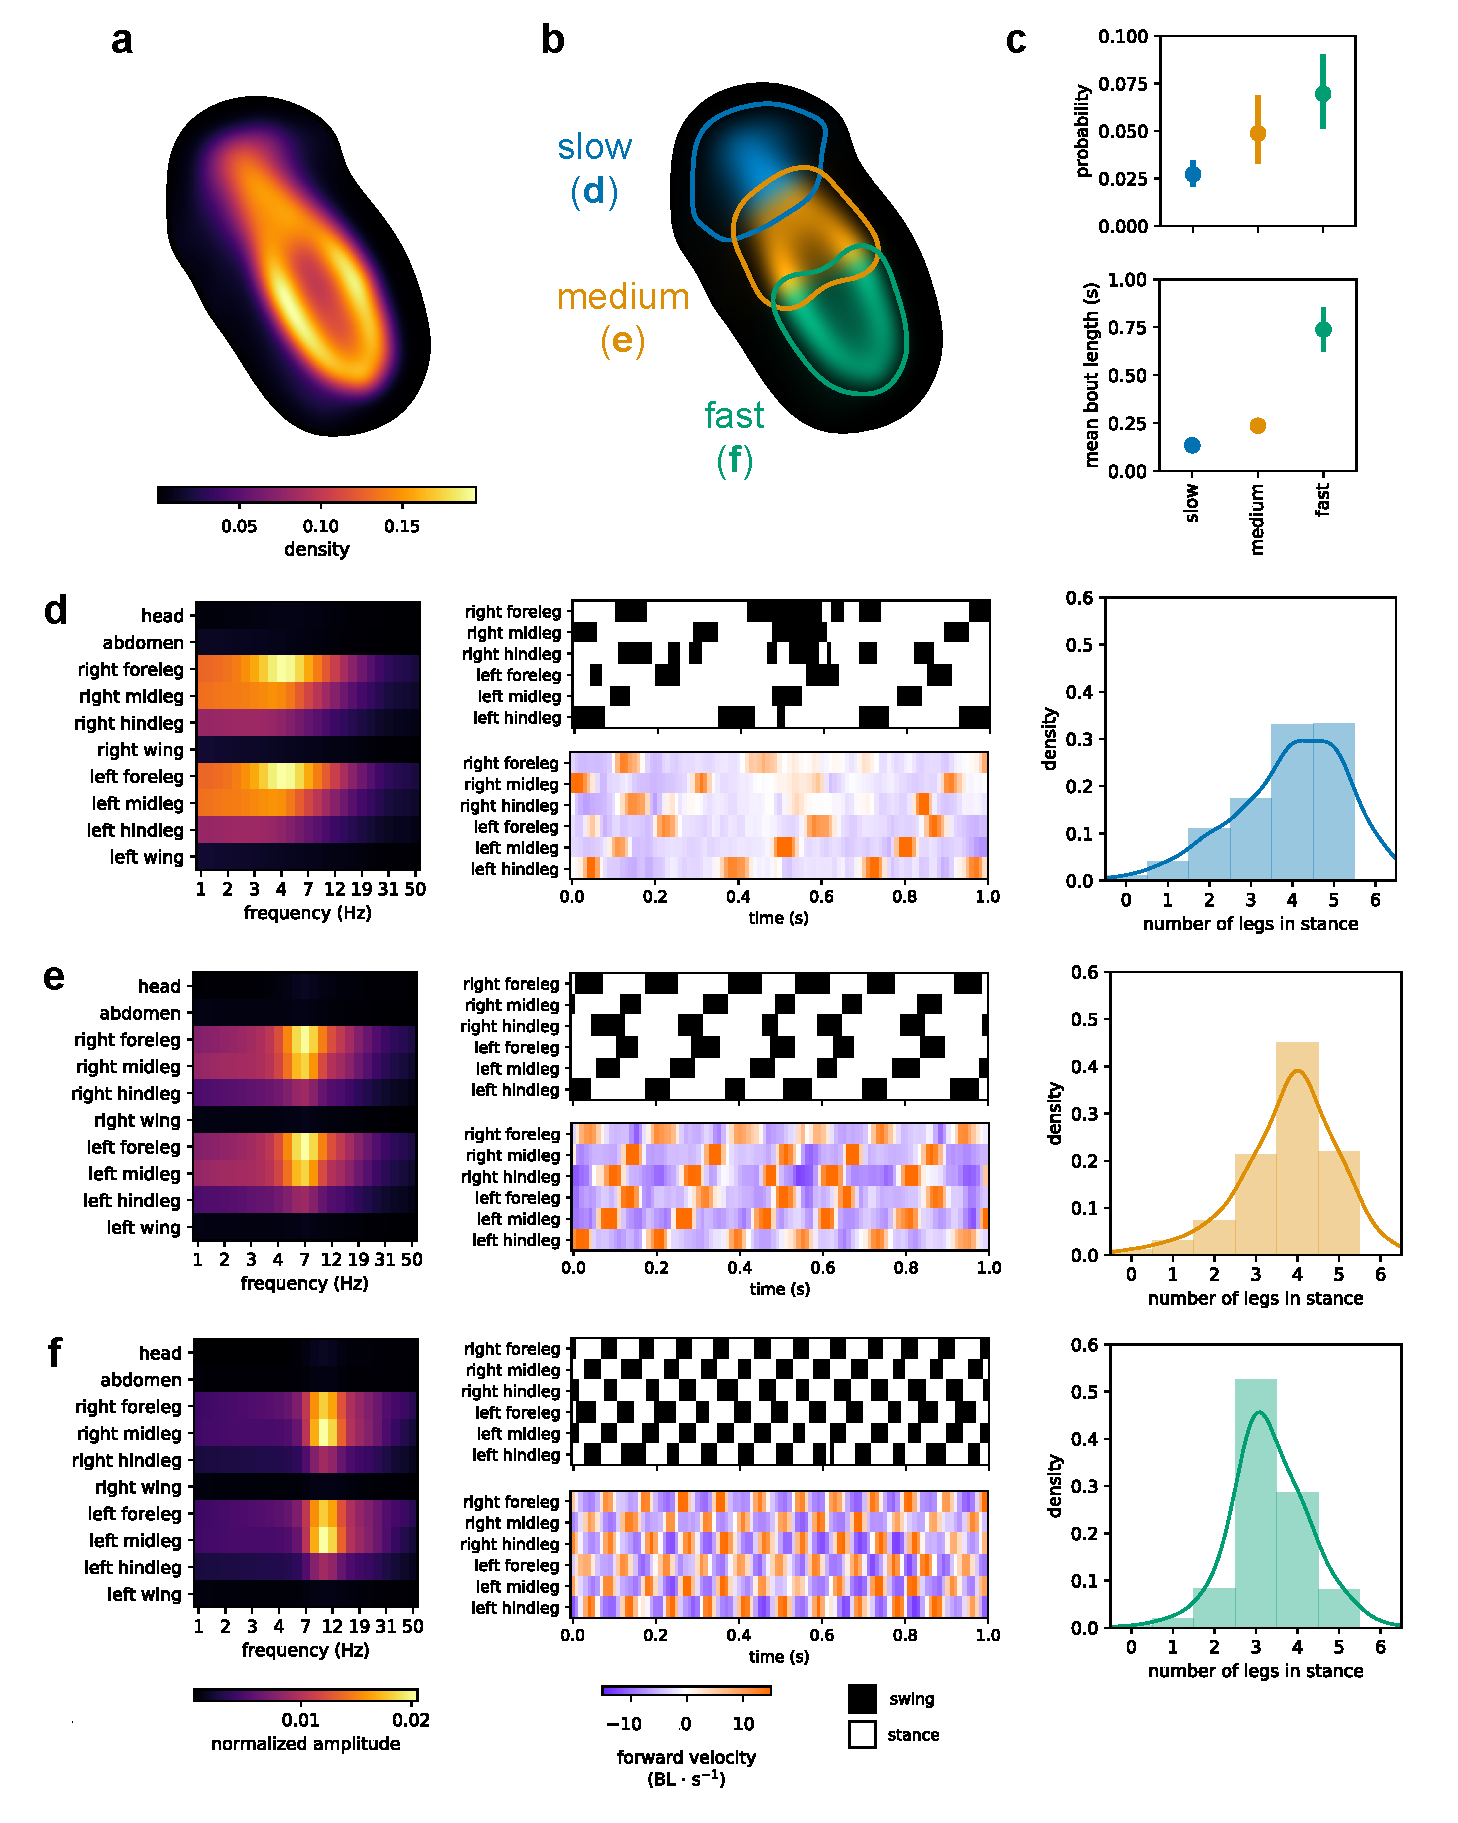
\includegraphics[width=0.9\textwidth]{Graving_IMPRS_Thesis/figures/locomotion_cluster_figure.pdf}
\bigskip
\caption{\textbf{Low-level locomotion clusters.} Visualizations describing the low-level clusters within the high-level locomotion cluster. \textbf{a-b}, The 2-D posterior probability density for the high-level cluster (\textbf{a}) and for each low-level cluster (\textbf{b}), where letters for each cluster label correspond to panels \textbf{d-f}. Contours are the largest 90\% probability density contour for each cluster distribution. \textbf{c}, Mean and 95\% bootstrap intervals of the marginal (stationary) probability and mean bout length for each low-level cluster (n = 59 per cluster). \textbf{d-f}, The mean spectrogram (left), example time segments (middle) showing forward velocity of each leg measured in body lengths (BL) per second and swing (forward velocity $> 0 \, \textrm{BL} \cdot \textrm{s}^{-1}$) or stance (forward velocity $\leq 0 \, \textrm{BL} \cdot \textrm{s}^{-1}$) classification, and histograms (right) showing the number of legs classified as stance in each timestep assigned to each cluster (n = 0.57 million for slow, \textbf{d}; n = 1.03 million for medium, \textbf{e}; and n = 1.47 million for fast, \textbf{f}) --- where the label for each panel in \textbf{d-f} corresponds to a cluster label in panel \textbf{b}. Example videos for these low-level clusters are shown in \ref{fig:locomotion_video}.}

\label{fig:locomotion_cluster_figure}

\end{figure}

\begin{figure}[!htb]
\centering
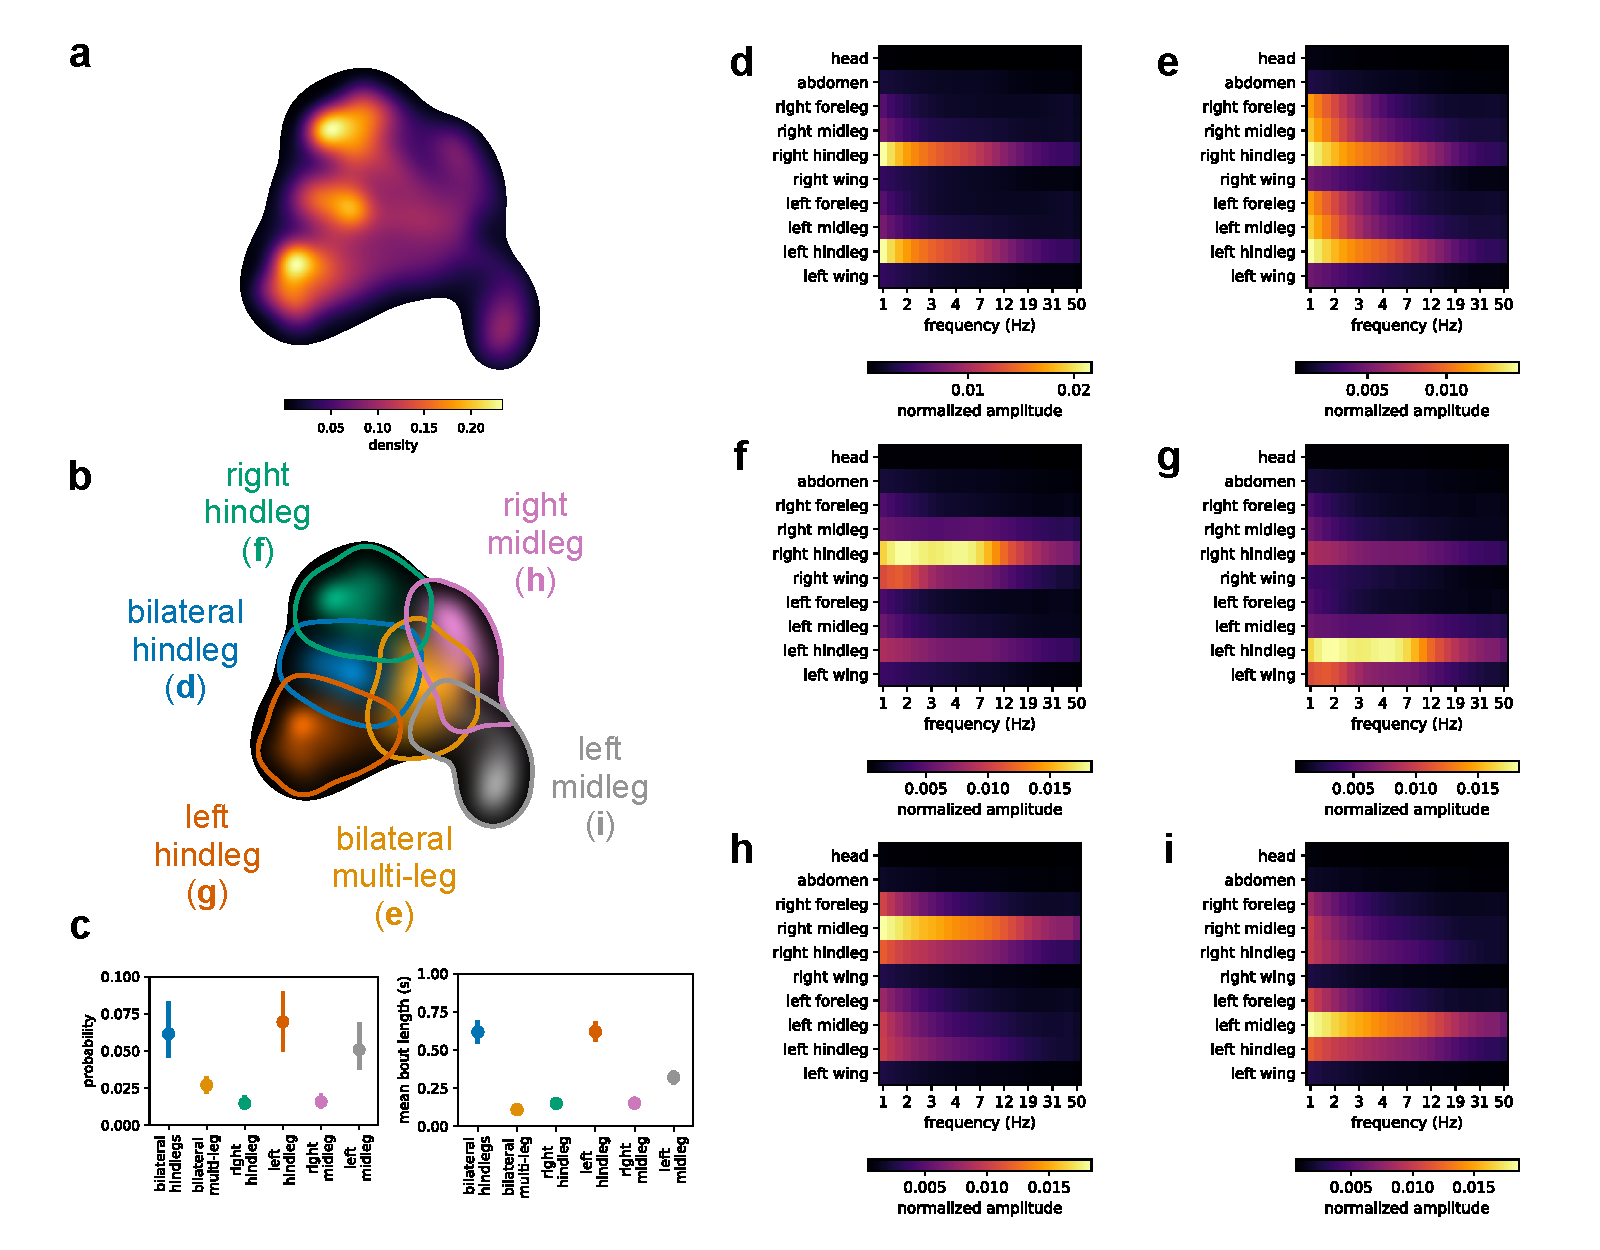
\includegraphics[width=1.0\textwidth]{Graving_IMPRS_Thesis/figures/posterior_cluster_figure.pdf}

\caption{  \textbf{Low-level posterior grooming clusters.} Visualizations describing the low-level clusters within the high-level posterior grooming cluster. \textbf{a-b}, The 2-D posterior probability density for the high-level cluster (\textbf{a}) and for each low-level cluster (\textbf{b}), where letters for each cluster label correspond to panels \textbf{d-i}. Contours are the largest 90\% probability density contour for each cluster distribution. \textbf{c}, Mean and 95\% bootstrap intervals of the marginal (stationary) probability and mean bout length for each low-level cluster (n = 59 per cluster). \textbf{d-i}, The mean spectrogram for each cluster --- where the label for each panel in \textbf{d-i} corresponds to a cluster label in panel \textbf{b}. Example videos for these low-level clusters are shown in \ref{fig:posterior_video}.}

\label{fig:posterior_cluster_figure}

\end{figure}


\begin{figure}[!htb]
\begin{center}
    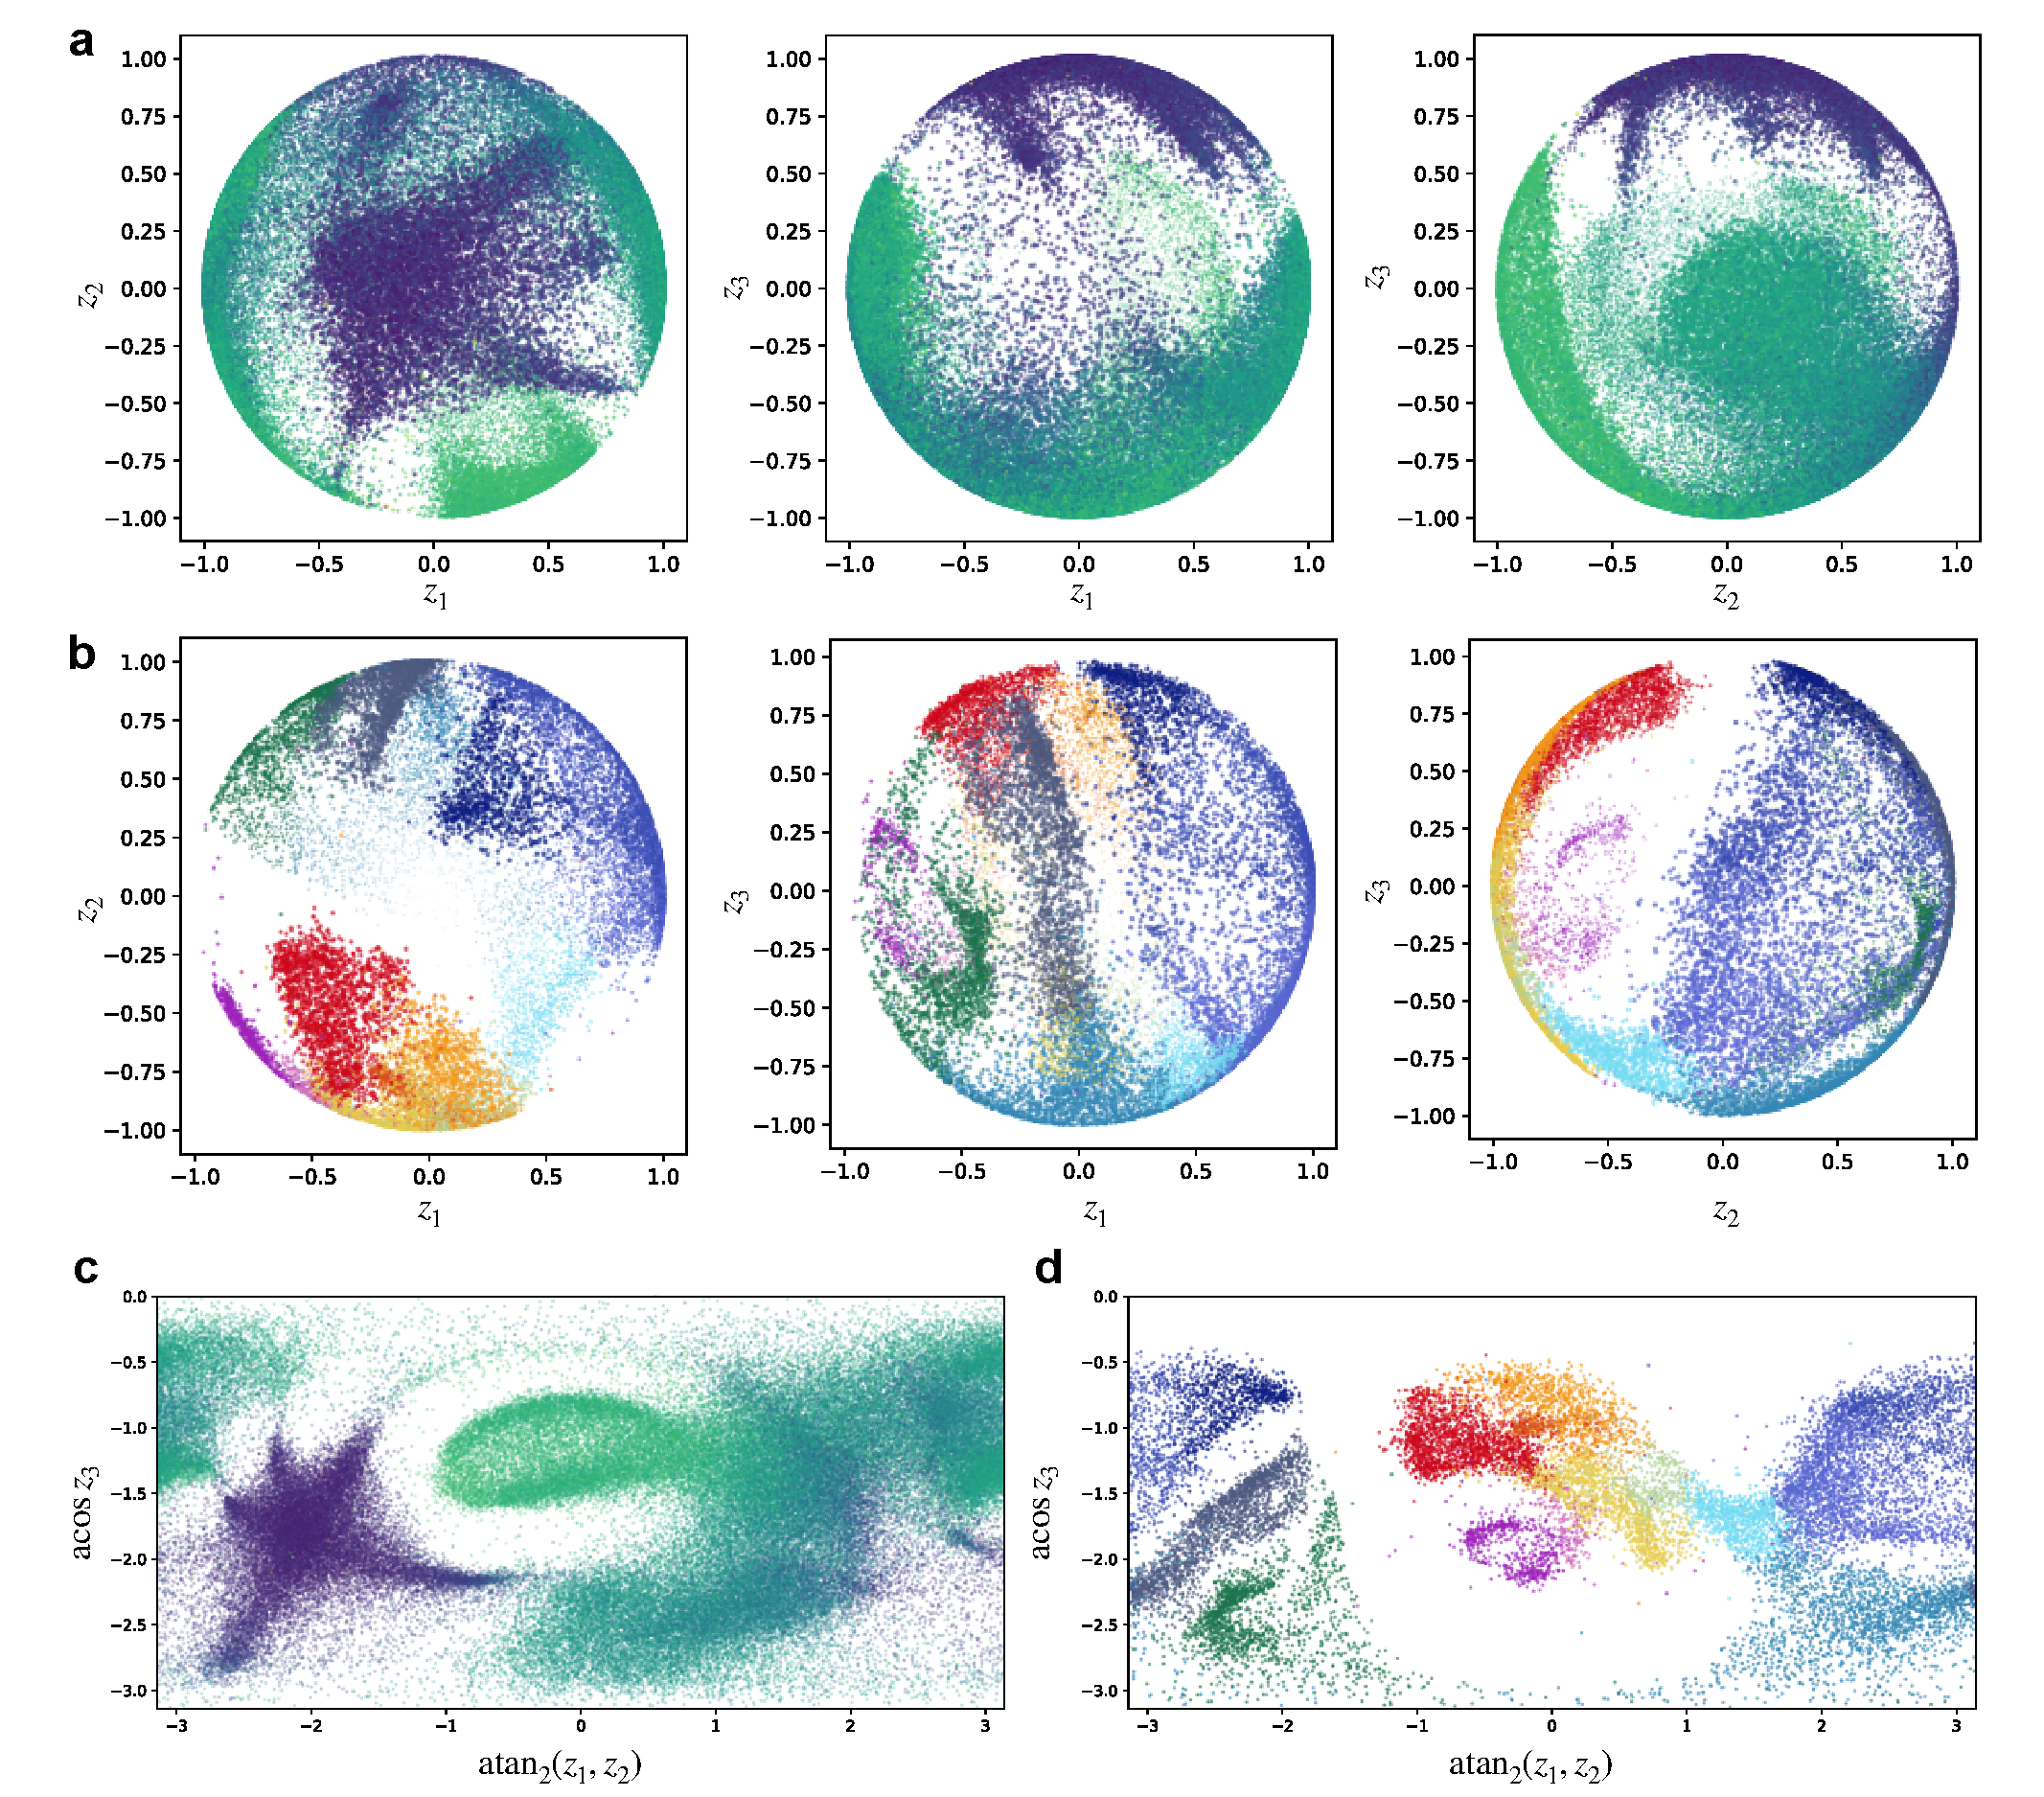
\includegraphics[width=\textwidth]{Graving_IMPRS_Thesis/figures/spherical_figure.pdf}
\end{center}

\caption{  \textbf{Spherical embeddings with von Mises-Fisher VAE-SNE}. \textbf{a-b}, Spherical embeddings using VAE-SNE with a von Mises-Fisher similarity kernel (Appendix \ref{appendix:spherical}) of the posture dynamics dataset (\textbf{a}; \ref{fig:spherical_embedding_posture_video}) from \cite{berman2014mapping, berman2016predictability, pereira2019fast} and the single-cell RNA-seq dataset (\textbf{b}; \ref{fig:spherical_embedding_rna_video}) from \cite{la2018rna}. \textbf{c-d}, Stereographic (planar) projections of the spherical embeddings from \textbf{a-b}. Colors for \textbf{a-d} are the same as in Fig. \ref{fig:embedded_data_figure} (total amplitude and cell type).}

\label{fig:spherical_figure} % \label works only AFTER \caption within figure environment

\end{figure}


\begin{figure}[!htb]
\begin{center}
    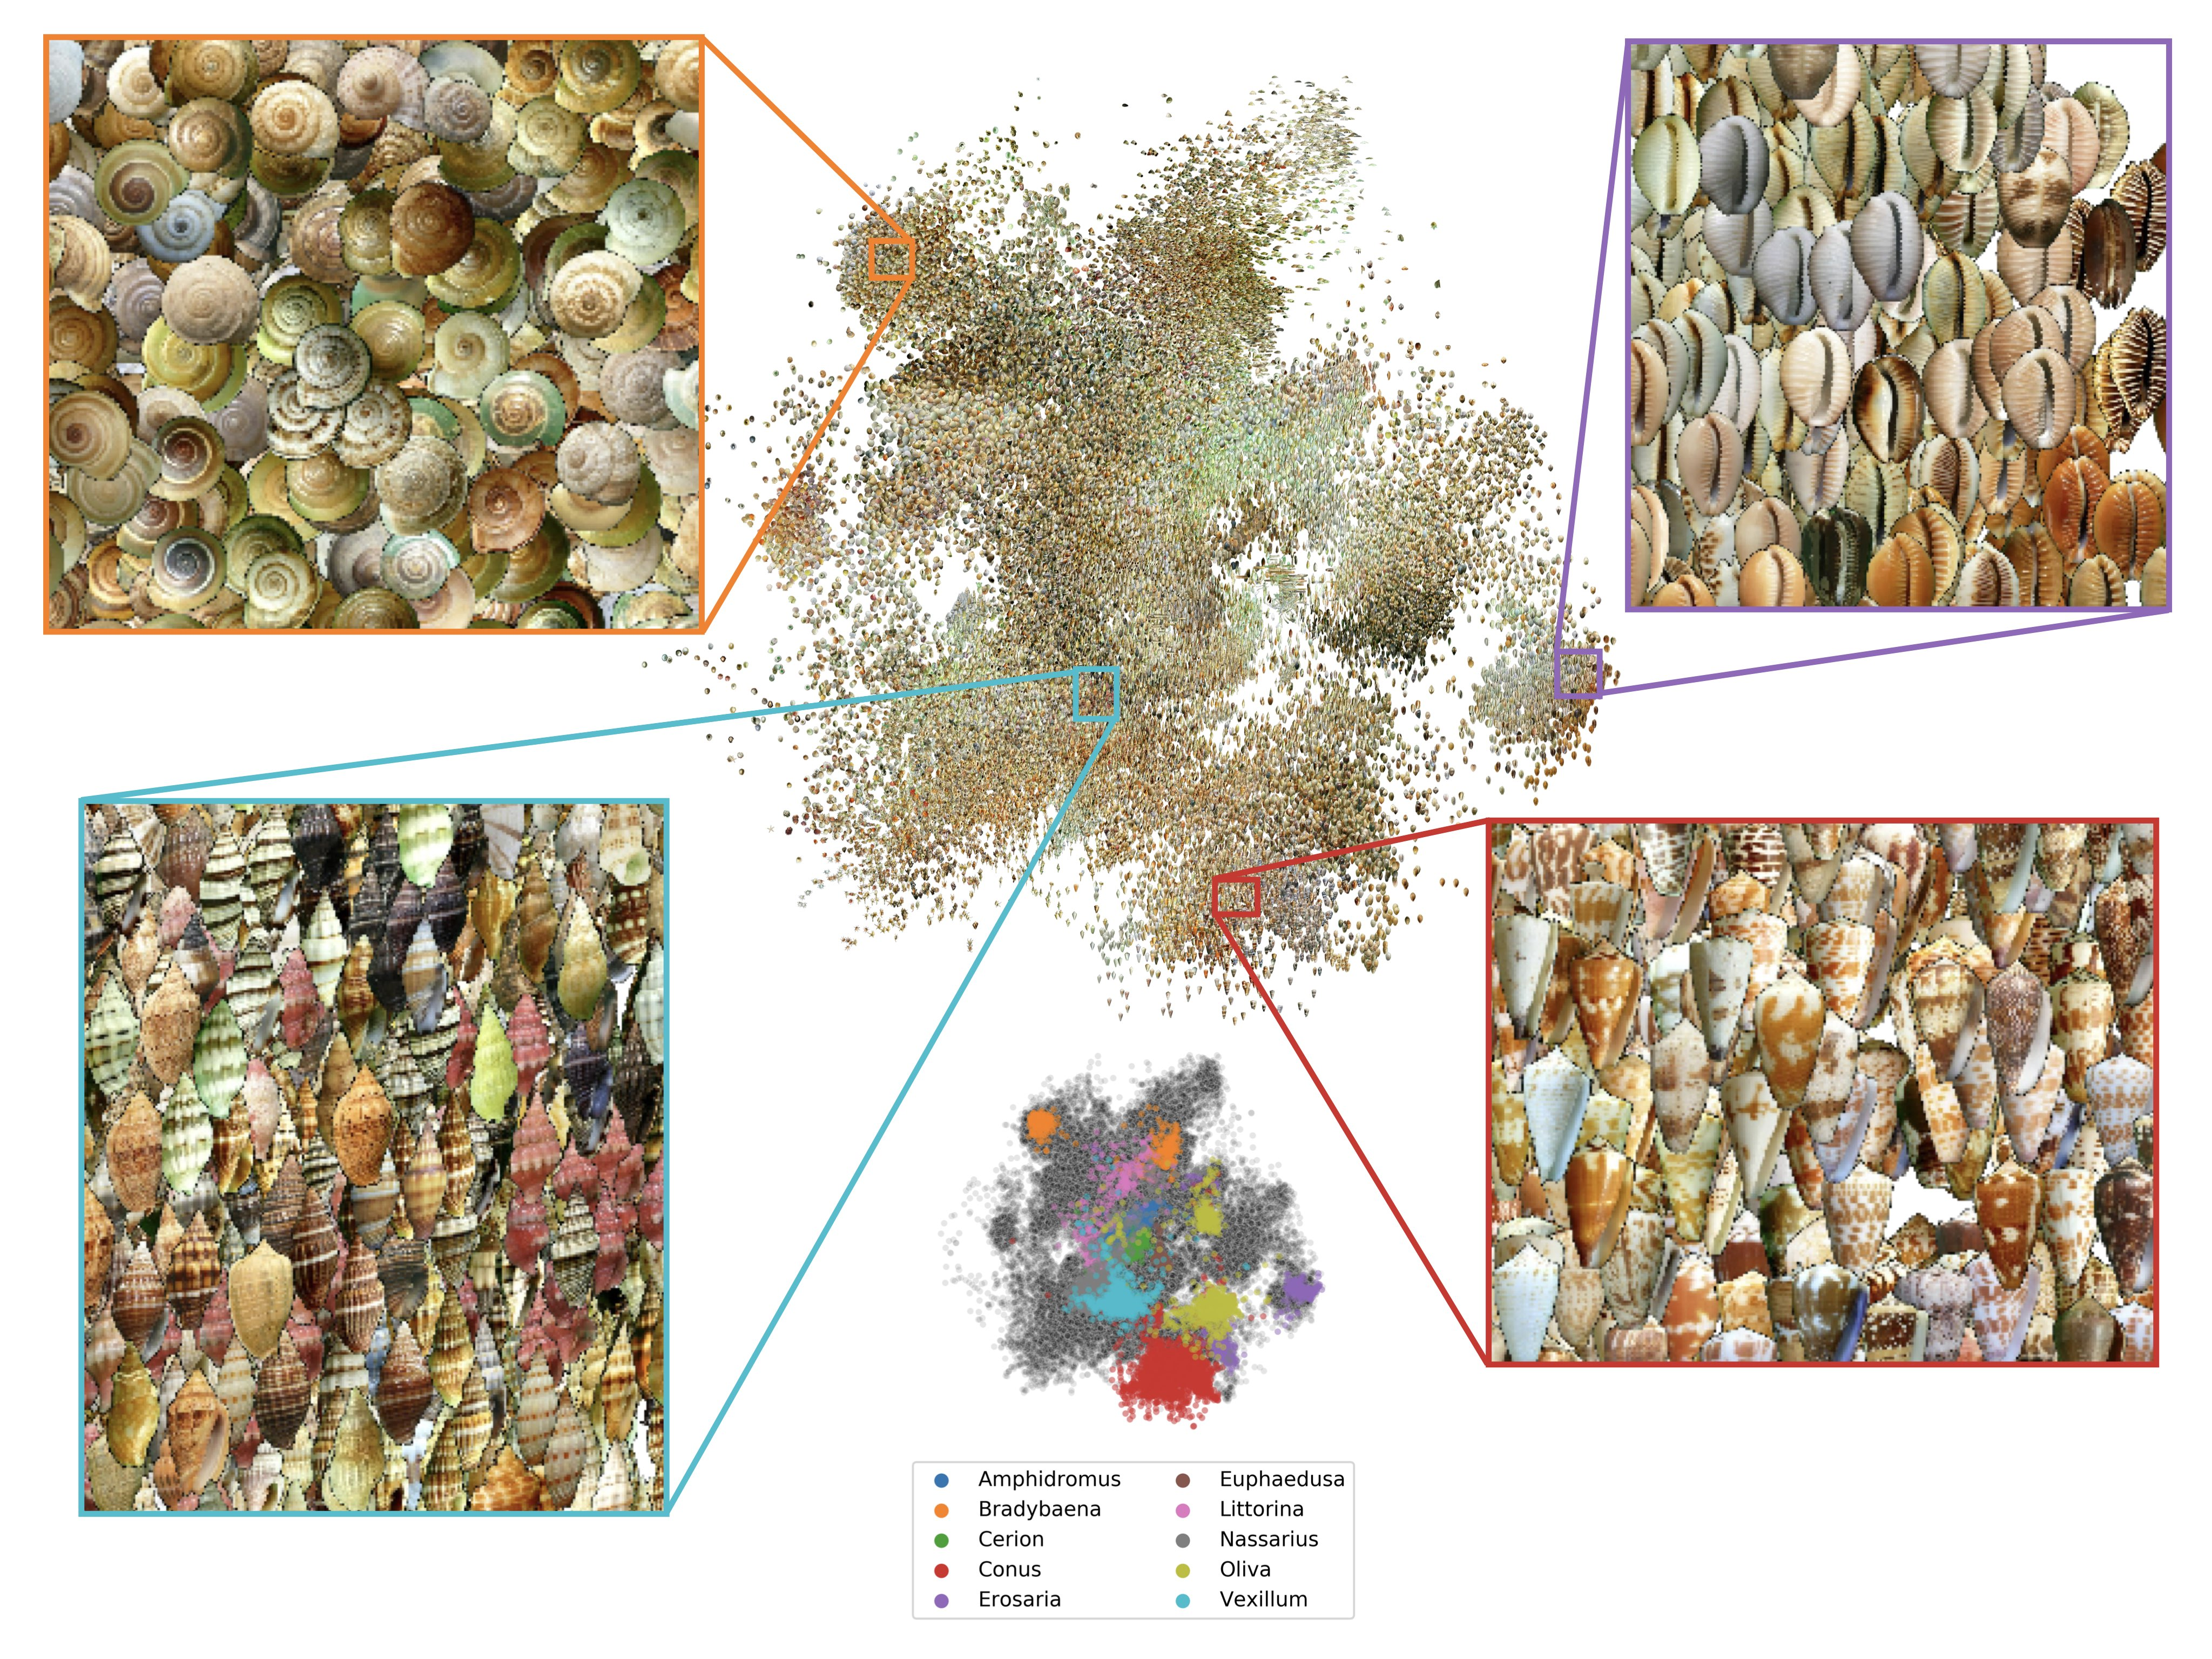
\includegraphics[width=\textwidth]{Graving_IMPRS_Thesis/figures/shell_figure.jpeg}
\end{center}

\caption{  \textbf{Embedding shell images}. Shell images from \cite{zhang2019shell} embedded in two dimensions using convolutional VAE-SNE. Insets illustrate example regions of perceptually similar images from the taxonomic genera \textit{Bradybaena} (land snails; top-left), \textit{Erosaria} (cowries; top-right), \textit{Vexillum} (sea snails; bottom-left), and \textit{Conus} (cone snails; bottom-right). Scatter plot (bottom-center) shows the 10 most common genera in the dataset.}

\label{fig:shell_figure} % \label works only AFTER \caption within figure environment

\end{figure}

\begin{figure}[!htb]
\begin{center}
    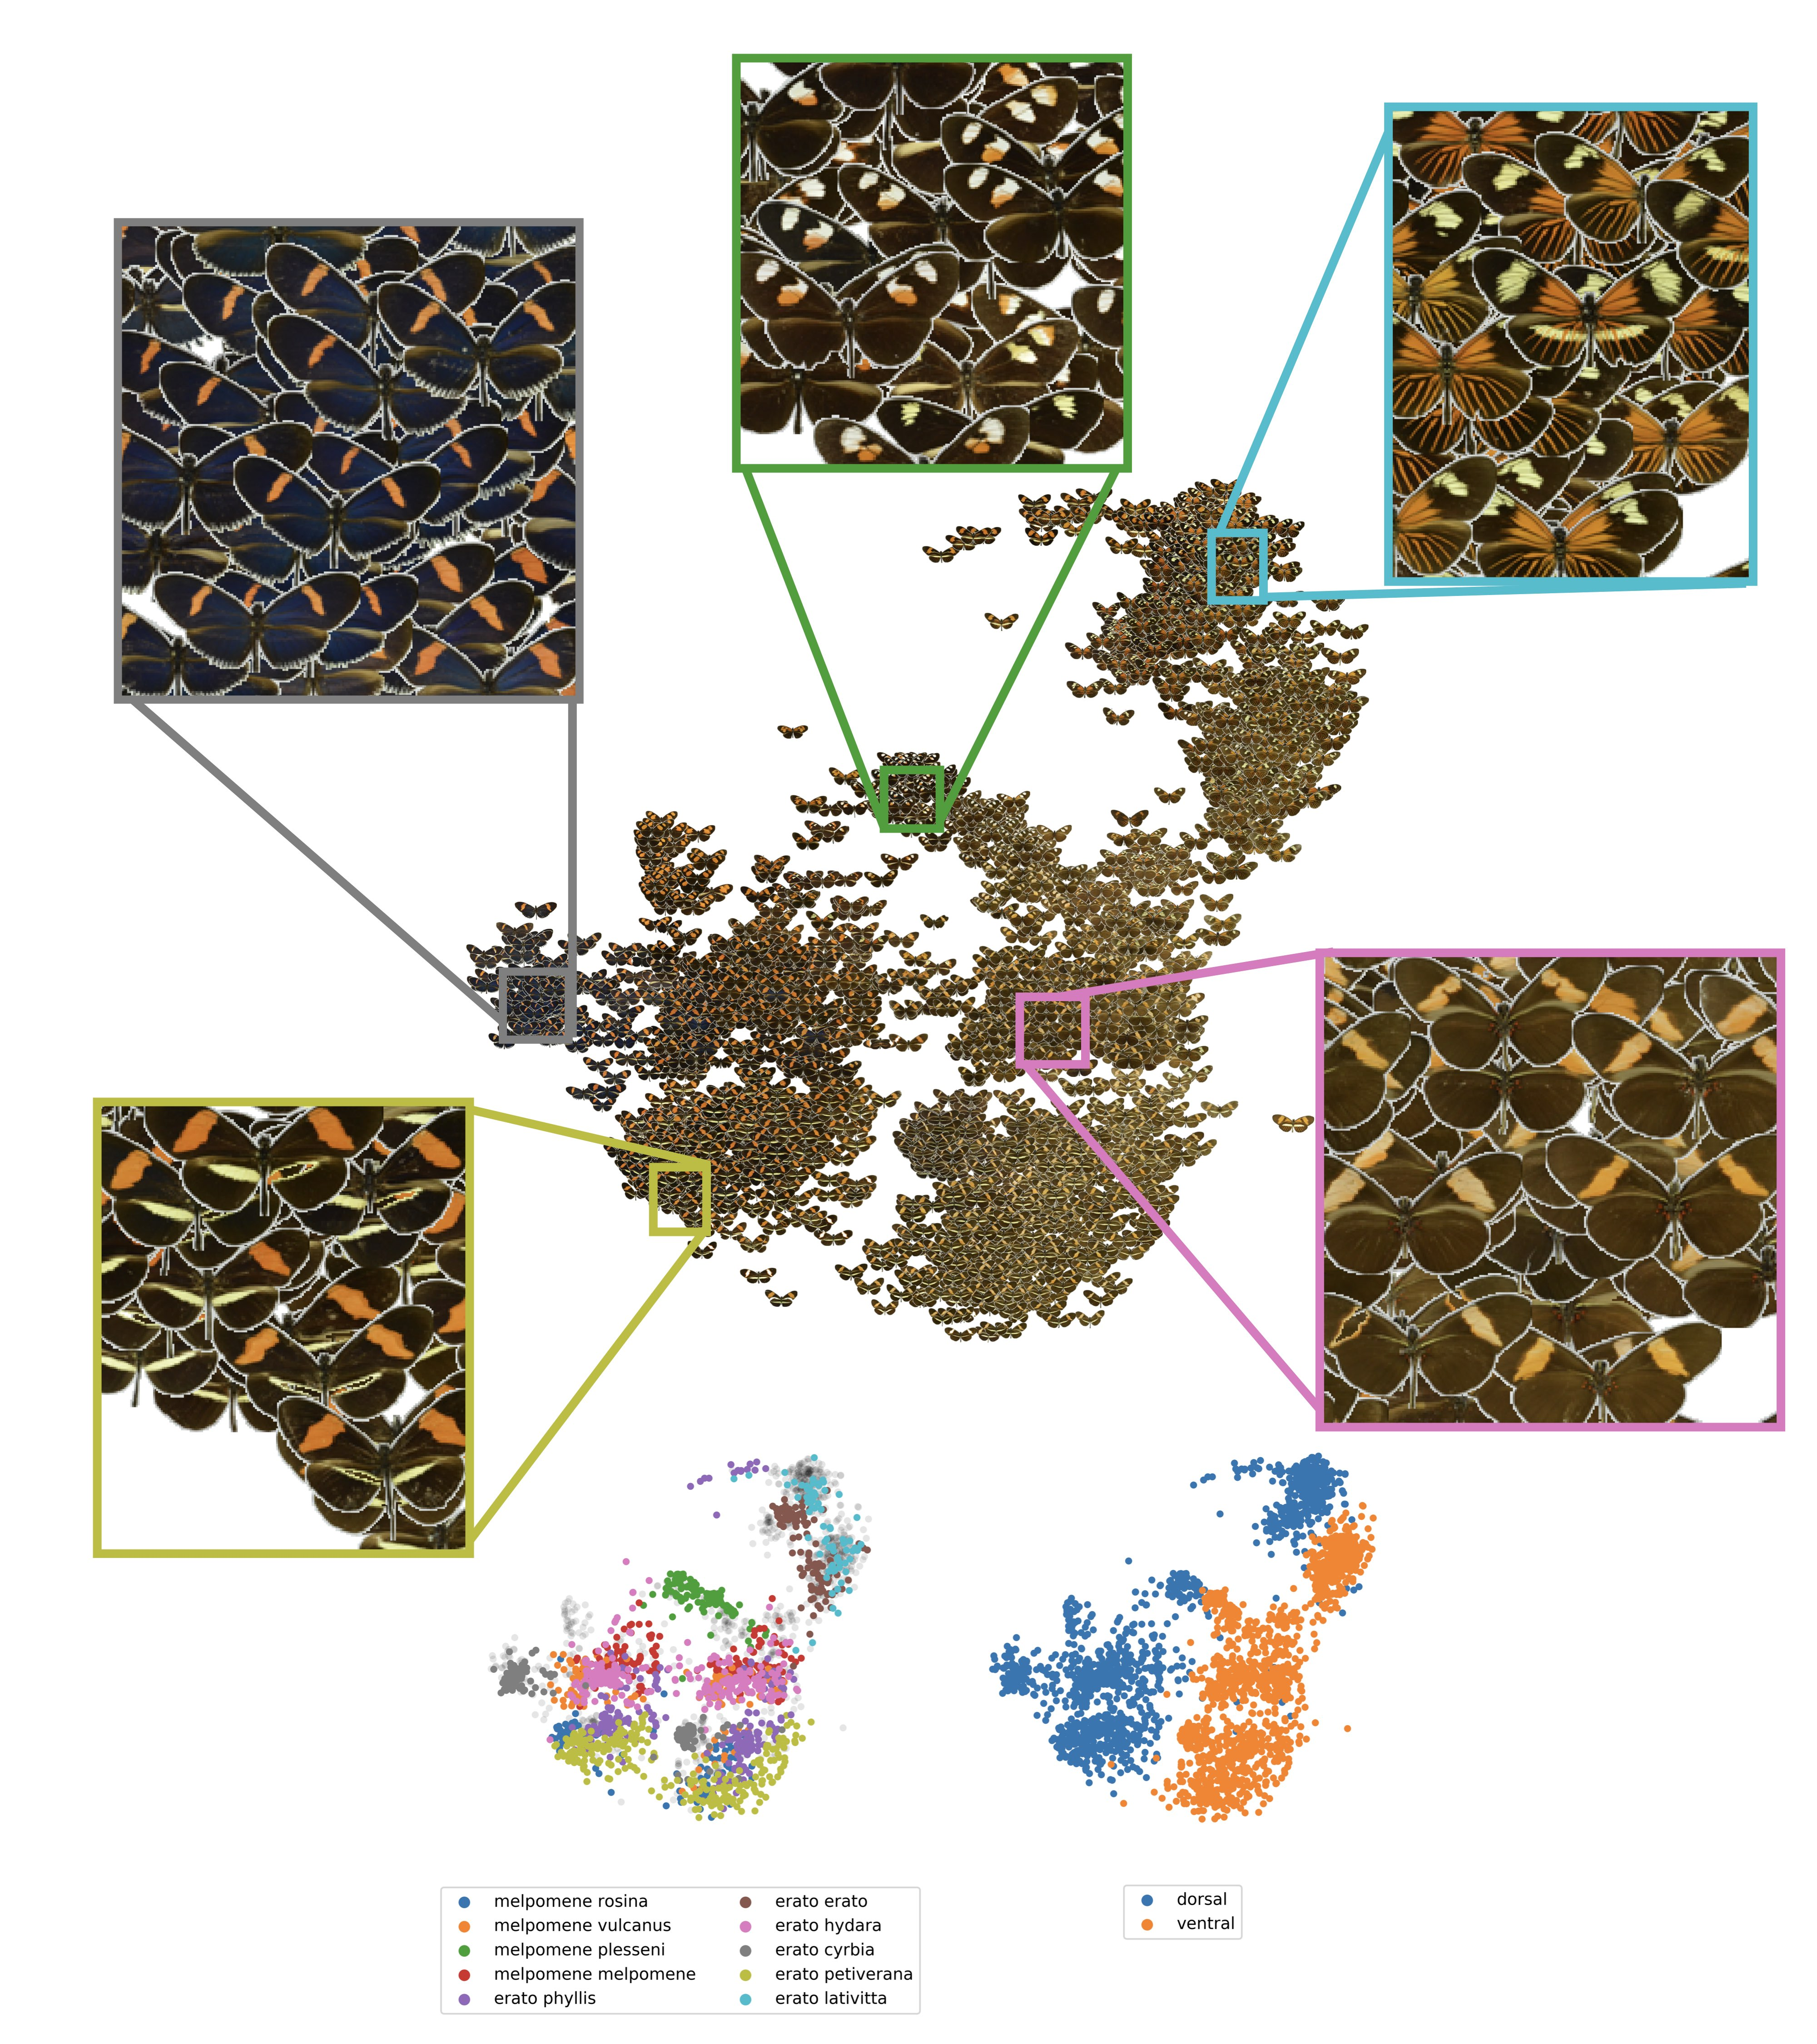
\includegraphics[width=\textwidth]{Graving_IMPRS_Thesis/figures/butterfly_figure.jpeg}
\end{center}

\caption{  \textbf{Embedding butterfly images}. Butterfly (\textit{Heliconius spp.}) images from \cite{cuthill2019deep} embedded in two dimensions using convolutional VAE-SNE. Insets show example regions of perceptually similar subspecies (top). Scatter plots (bottom) show labels for the 10 most common subspecies in the dataset (bottom-left) and the image viewpoint relative to the specimen's dorso-ventral body axis (bottom-right).}

\label{fig:butterfly_figure} % \label works only AFTER \caption within figure environment

\end{figure}

\clearpage
\setcounter{figure}{0}
\renewcommand{\thefigure}{Video S\arabic{figure}}

\begin{figure}[!htb]
\caption{
\textbf{Video segments labeled with VAE-SNE}. Randomly selected video segments ($1/2 \times$ speed) labeled with VAE-SNE illustrating the temporal dynamics of movements through the behavioral space and transitions between high-level clusters within the distribution. \textbf{a}, \href{https://youtu.be/JlbSdKzvLfk}{https://youtu.be/JlbSdKzvLfk}; \textbf{b}, \href{https://youtu.be/uWScG_UuzRQ}{https://youtu.be/uWScG\_UuzRQ}; \textbf{c}, \href{https://youtu.be/T8e_JSoCwMA}{https://youtu.be/T8e\_JSoCwMA}
}
\label{fig:sequences_video}
\end{figure}


\begin{figure}[!htb]
\caption{
\textbf{Samples from the locomotion cluster}. Randomly sampled videos ($1/3 \times$ speed) from the locomotion cluster showing: \textbf{a}, slow walking (\href{https://youtu.be/hB3JIRF2JGQ}{https://youtu.be/hB3JIRF2JGQ}); \textbf{b}, medium walking (\href{https://youtu.be/kNHGJypOGhs}{https://youtu.be/kNHGJypOGhs}); and \textbf{c}, fast walking (\href{https://youtu.be/A2sLtgYhHGc}{https://youtu.be/A2sLtgYhHGc}). Red lines show the posture tracking data for all 32 keypoints.
}
\label{fig:locomotion_video}
\end{figure}

\begin{figure}[!htb]
\caption{
\textbf{Samples from the anterior grooming cluster}. Randomly sampled videos ($1/3 \times$ speed) from one of the anterior grooming clusters (\href{https://youtu.be/0MT3lb2bJro}{https://youtu.be/0MT3lb2bJro}). Red lines show the posture tracking data for all 32 keypoints.
}
\label{fig:anterior_video}
\end{figure}

\begin{figure}[!htb]
\caption{
\textbf{Samples from the posterior grooming cluster}. Randomly sampled videos ($1/3 \times$ speed) from the posterior grooming cluster showing: \textbf{a}, bilateral hindleg grooming (\href{https://youtu.be/O_Tyf4pEQMo}{https://youtu.be/O\_Tyf4pEQMo}); \textbf{b}, right hindleg grooming (\href{https://youtu.be/VTIwZp6d6b4}{https://youtu.be/VTIwZp6d6b4}); \textbf{b}, left midleg grooming (\href{https://youtu.be/0vJvAINbfjw}{https://youtu.be/0vJvAINbfjw}). Red lines show the posture tracking data for all 32 keypoints. 
}
\label{fig:posterior_video}

\end{figure}

\begin{figure}[!htb]
\caption{
\textbf{Samples from the wing movements cluster}. Randomly sampled videos ($1/3 \times$ speed) from the wing movements cluster showing: \textbf{a}, wing extensions (\href{https://youtu.be/lE31SeJ7ehY}{https://youtu.be/lE31SeJ7ehY}); and \textbf{b}, wing flicks (\href{https://youtu.be/nsgnFbrk090}{https://youtu.be/nsgnFbrk090}). Red lines show the posture tracking data for all 32 keypoints.
}
\label{fig:wing_video}
\end{figure}

\begin{figure}[!htb]
\caption{
\textbf{Samples from the small/slow leg movements cluster}. Randomly sampled videos ($1/3 \times$ speed) from the small/slow leg movement cluster showing: \textbf{a}, small leg movements (\href{https://youtu.be/ARkH1uvPBnQ}{https://youtu.be/ARkH1uvPBnQ}); \textbf{b}, slow leg movements (\href{https://youtu.be/hwL7ovNjbBQ}{https://youtu.be/hwL7ovNjbBQ}); \textbf{c}, small left midleg movements (\href{https://youtu.be/o8vxtgwzx9Q}{https://youtu.be/o8vxtgwzx9Q}) Red lines show the posture tracking data for all 32 keypoints. 
}
\label{fig:slow_video}
\end{figure}

\begin{figure}[!htb]
\caption{
\textbf{Samples from the idle cluster}. Randomly sampled videos ($1/3 \times$ speed) from the idle cluster (\href{https://youtu.be/0wbdqmuCe_g}{https://youtu.be/0wbdqmuCe\_g}). Red lines show the posture tracking data for all 32 keypoints.}
\label{fig:idle_video}
\end{figure}

\begin{figure}[!htb]
\caption{
\textbf{Spherical embedding of the posture dynamics dataset}. Rotating view of the posture dynamics dataset (\href{https://youtu.be/QcDUlQUOvdo}{https://youtu.be/QcDUlQUOvdo}) from \cite{berman2014mapping, berman2016predictability, pereira2019fast} embedded on a 3-D sphere using von Mises-Fisher VAE-SNE. Colors are the same as in Fig. \ref{fig:embedded_data_figure} (total amplitude).
}
\label{fig:spherical_embedding_posture_video}
\end{figure}

\begin{figure}[!htb]
\caption{
\textbf{Spherical embedding of the single-cell RNA-seq dataset}. Rotating view of the single-cell RNA-seq dataset (\href{https://youtu.be/jyIWB6-qye0}{https://youtu.be/jyIWB6-qye0}) from \cite{la2018rna} embedded on a 3-D sphere using von Mises-Fisher VAE-SNE. Colors are the same as in Fig. \ref{fig:embedded_data_figure} (cell type).
}
\label{fig:spherical_embedding_rna_video}
\end{figure}

\section[VAEs and the ELBO]{Variational autoencoders and the evidence lower bound}


\subsection{VAEs as approximate Bayesian inference}
\label{appendix:vae}
As is common to most dimensionality reduction algorithms, we seek to model a high-dimensional data distribution $p(\mathbf{x})$ using a low dimensional latent distribution $p(\mathbf{z})$. Variational autoencoders (VAEs) are one such model that combines both modeling and inference by defining a joint distribution between a latent variable $\mathbf{z}$ and observed samples $\mathbf{x}$. We can accomplish this using a generative model that maps samples from the low-dimensional latent distribution to the high-dimensional data distribution using a set of shared parameters $\boldsymbol{\theta}$, which can take the form of a deep neural network model $p_{\boldsymbol{\theta}}(\mathbf{x} | \mathbf{z}) = \mathrm{DNN}_{\boldsymbol{\theta}}(\mathbf{z})$ with some prior over latent distribution $p_{\boldsymbol{\theta}}(\mathbf{z})$. We then wish to find the model parameters $\boldsymbol{\theta}$ that maximize the joint likelihood, which can be written as:

\begin{equation}
     \argmax_{\boldsymbol{\theta}} p_{\boldsymbol{\theta}}(\mathbf{x}, \mathbf{z}) = \argmax_{\boldsymbol{\theta}} p_{\boldsymbol{\theta}}(\mathbf{x} | \mathbf{z})p_{\boldsymbol{\theta}}(\mathbf{z}).
\end{equation}
Although, to compute the low-dimensional distribution for the data, we then need to derive the latent posterior for the model $p_{\boldsymbol{\theta}}(\mathbf{z} | \mathbf{x})$. This can be derived from the likelihood using Bayes' rule:

\begin{equation}
      p_{\boldsymbol{\theta}}(\mathbf{z}|\mathbf{x}) = \frac{p_{\boldsymbol{\theta}}(\mathbf{x} | \mathbf{z})p_{\boldsymbol{\theta}}(\mathbf{z})} {p_{\boldsymbol{\theta}}(\mathbf{x})}.
      \label{eq:intractable_integral}
\end{equation}
However, computing the integral in Eq. \ref{eq:intractable_integral} $p_{\boldsymbol{\theta}}(\mathbf{x}) = \int p_{\boldsymbol{\theta}}(\mathbf{x} | \mathbf{z})p_{\boldsymbol{\theta}}(\mathbf{z})\, d\mathbf{z}$ is not tractable in practice. Therefore, we require a way to approximate this latent posterior distribution, which is the exact problem for which VAEs provide a tractable solution.

Like other VAE models \citep{kingma2013vae, kingma2014semi, burda2015iwae, dilokthanakul2016gmvae, ding2018scvis, dieng2019avoiding}, VAE-SNE performs dimensionality reduction by nonlinearly mapping observed high-dimensional data vectors $\mathbf{x}$ to a low-dimensional embedding $\mathbf{z}$ using a deep neural network ($\mathrm{DNN}$) as an encoder function $\mathrm{DNN}_{\boldsymbol{\phi}} : \mathbf{x} \to \mathbf{z}$ (Eq. \ref{eq:encoder}) with the goal of learning an approximate posterior over the latent distribution $q_{\boldsymbol{\phi}}(\mathbf{z} | \mathbf{x})$ (Eq. \ref{eq:approx}), where the parameters of the approximate posterior are learned as a function of the data (Eq. \ref{eq:encoder}) and the encoder parameters $\boldsymbol{\phi}$ are then shared across observed samples --- known as \textit{amortization}. The model then maps latent vectors sampled from the low-dimensional embedding (Eq. \ref{eq:sample}) to reconstruct the original high-dimensional space $\mathrm{DNN}_{\boldsymbol{\theta}} : \mathbf{z} \to \tilde{\mathbf{x}}$ (Eq. \ref{eq:recon}) using a generative decoder function we defined earlier (rewritten in Eq. \ref{eq:likelihood}). More precisely:

\begin{subequations}
\begin{align}
    \tilde{\mathbf{x}} &\sim
    p_{\boldsymbol{\theta}}(\mathbf{x} | \mathbf{z}) \label{eq:recon}\\
    p_{\boldsymbol{\theta}}(\mathbf{x} | \mathbf{z}) &= \mathcal{L} \left( \mathbf{x} | \mathrm{DNN}_{\boldsymbol{\theta}}(\mathbf{z}) \right) \label{eq:likelihood}\\
    \mathbf{z} &\sim
    q_{\boldsymbol{\phi}}(\mathbf{z} | \mathbf{x})\label{eq:sample}\\
    q_{\boldsymbol{\phi}}(\mathbf{z} | \mathbf{x}) &= \mathcal{N}(\mathbf{z} | \boldsymbol{\mu}, \mathrm{diag}(\boldsymbol{\sigma}^2)) \label{eq:approx}\\
    (\boldsymbol{\mu}, \log \boldsymbol{\sigma}^2) &= \mathrm{DNN}_{\boldsymbol{\phi}}(\mathbf{x})\label{eq:encoder}
\end{align}
\end{subequations}
where $\mathcal{L}(\mathbf{x}| \cdot)$ is a user-selected likelihood function parameterized by the decoder function $\mathrm{DNN}_{\boldsymbol{\theta}}(\mathbf{z})$, and $\mathcal{N}(\cdot | \boldsymbol{\mu}, \mathrm{diag}(\boldsymbol{\sigma}^2))$ is a multivariate Gaussian whose parameters $\boldsymbol{\mu}$ and $\boldsymbol{\boldsymbol{\sigma}^2}$ are a specified by the encoder function $\mathrm{DNN}_{\boldsymbol{\phi}}(\mathbf{x})$. 

\subsection{Deriving the evidence lower bound}
\label{appendix:elbo}
After defining the generative model, we then wish to optimize the parameters of the encoder $\boldsymbol{\phi}$ and decoder $\boldsymbol{\theta}$ --- given a set of observed samples from a data distribution $\mathbf{x} \sim p(\mathbf{x})$ --- so that the approximate posterior distribution $q_{\boldsymbol{\phi}}(\mathbf{z} | \mathbf{x})$ matches closely with the true latent posterior from the generative decoder, or $q_{\boldsymbol{\phi}}(\mathbf{z} | \mathbf{x}) \approx p_{\boldsymbol{\theta}}(\mathbf{z} | \mathbf{x})$. In other words, we wish to minimize the divergence between the two distributions, or:

\begin{equation}
    \label{eq:posterior_divergence}
    \argmin_{\boldsymbol{\theta}, \boldsymbol{\phi}} \mathbb{KL}[q_{\boldsymbol{\phi}}(\mathbf{z} | \mathbf{x}) \| p_{\boldsymbol{\theta}}(\mathbf{z} | \mathbf{x})] = \argmin_{\boldsymbol{\theta}, \boldsymbol{\phi}} \int q_{\boldsymbol{\phi}}(\mathbf{z} | \mathbf{x}) \log \frac{q_{\boldsymbol{\phi}}(\mathbf{z} | \mathbf{x})}{p_{\boldsymbol{\theta}}(\mathbf{z} | \mathbf{x})} \, d{\mathbf{z}}.
\end{equation}
However, as we have already established, computing the true posterior is intractable, so researchers have derived a lower bound known as the evidence lower bound, or $\mathrm{ELBO}$ \citep{kingma2013vae}, to approximate this objective. The $\mathrm{ELBO}$ can be derived directly from Eq.\ref{eq:posterior_divergence} \citep{adams2020}, which is written as:

\begin{subequations}
    \begin{align}
    \mathbb{KL}[q_{\boldsymbol{\phi}}(\mathbf{z} | \mathbf{x}) \| p_{\boldsymbol{\theta}}(\mathbf{z} | \mathbf{x})] &= \int q_{\boldsymbol{\phi}}(\mathbf{z} | \mathbf{x}) \log \frac{q_{\boldsymbol{\phi}}(\mathbf{z} | \mathbf{x})}{p_{\boldsymbol{\theta}}(\mathbf{z} | \mathbf{x})} \, d\mathbf{z} \\
    &= \log p_{\boldsymbol{\theta}}(\mathbf{x}) + \int q_{\boldsymbol{\phi}}(\mathbf{z} | \mathbf{x}) \log \frac{q_{\boldsymbol{\phi}}(\mathbf{z} | \mathbf{x})}{p_{\boldsymbol{\theta}}(\mathbf{z} | \mathbf{x})} \, d{\mathbf{z}} - \log p_{\boldsymbol{\theta}}(\mathbf{x}) \\
    &= \log p_{\boldsymbol{\theta}}(\mathbf{x}) + \int q_{\boldsymbol{\phi}}(\mathbf{z} | \mathbf{x}) \log \frac{q_{\boldsymbol{\phi}}(\mathbf{z} | \mathbf{x})}{p_{\boldsymbol{\theta}}(\mathbf{z} | \mathbf{x})} \, d{\mathbf{z}} - \int \log q_{\boldsymbol{\phi}}(\mathbf{z} | \mathbf{x}) p_{\boldsymbol{\theta}}(\mathbf{x}) \, d{\mathbf{z}} \\
    &= \log p_{\boldsymbol{\theta}}(\mathbf{x}) + \int q_{\boldsymbol{\phi}}(\mathbf{z} | \mathbf{x}) \log \frac{q_{\boldsymbol{\phi}}(\mathbf{z} | \mathbf{x})}{p_{\boldsymbol{\theta}}(\mathbf{z} | \mathbf{x})p_{\boldsymbol{\theta}}(\mathbf{x})} \, d{\mathbf{z}} \\
    &= \log p_{\boldsymbol{\theta}}(\mathbf{x}) -\mathbb{E}_{    q_{\boldsymbol{\phi}}(\mathbf{z} | \mathbf{x})}\left[\log\frac{p_{\boldsymbol{\theta}}(\mathbf{x}, \mathbf{z})}{q_{\boldsymbol{\phi}}(\mathbf{z} | \mathbf{x})}\right]  \\
    &= \log p_{\boldsymbol{\theta}}(\mathbf{x}) -\mathrm{ELBO}(\boldsymbol{\theta}, \boldsymbol{\phi}).
\end{align}
\end{subequations}
Because the Kullback-Leibler divergence is strictly non-negative, the $\mathrm{ELBO}$ is then a lower bound on the log marginal likelihood. However, The $\mathrm{ELBO}$ can also be derived by applying Jensen's inequality, as is more common in the literature \citep{kingma2013vae}, to directly calculate a lower bound on the log marginal likelihood, or:

\begin{subequations}
\begin{align}
    \log p_{\boldsymbol{\theta}}(\mathbf{x}) &= \log \int p_{\boldsymbol{\theta}}(\mathbf{x}, \mathbf{z}) \, d\mathbf{z} \\
    &= \log \int p_{\boldsymbol{\theta}}(\mathbf{x}, \mathbf{z}) \frac{q_{\boldsymbol{\phi}}(\mathbf{z} | \mathbf{x})}{q_{\boldsymbol{\phi}}(\mathbf{z} | \mathbf{x})} \, d\mathbf{z} \\
    &= \log \mathbb{E}_{q_{\boldsymbol{\phi}}(\mathbf{z} | \mathbf{x})}\left[\frac{p_{\boldsymbol{\theta}}(\mathbf{x}, \mathbf{z})}{q_{\boldsymbol{\phi}}(\mathbf{z} | \mathbf{x})}\right] \\
    &\geq \mathbb{E}_{    q_{\boldsymbol{\phi}}(\mathbf{z} | \mathbf{x})}\left[\log\frac{p_{\boldsymbol{\theta}}(\mathbf{x}, \mathbf{z})}{q_{\boldsymbol{\phi}}(\mathbf{z} | \mathbf{x})}\right] = \mathrm{ELBO}(\boldsymbol{\theta}, \boldsymbol{\phi}).
\end{align}
\end{subequations}

To learn the latent distribution given the model and the data, the $\mathrm{ELBO}$ is then maximized to optimize the model parameters. Here we write this as a minimization of the negative $\mathrm{ELBO}$, which can be further decomposed into separate terms for the log-likelihood and the divergence between the approximate posterior and the prior over the latent distribution, or:

\begin{subequations}
\begin{align}
    \argmin_{\boldsymbol{\theta}, \boldsymbol{\phi}}-\mathrm{ELBO}(\boldsymbol{\theta}, \boldsymbol{\phi}) &= \argmin_{\boldsymbol{\theta}, \boldsymbol{\phi}} \mathbb{E}_{    q_{\boldsymbol{\phi}}(\mathbf{z} | \mathbf{x})}\left[ \log\frac{q_{\boldsymbol{\phi}}(\mathbf{z} | \mathbf{x})}{p_{\boldsymbol{\theta}}(\mathbf{x}, \mathbf{z})}\right] \\
    &= \argmin_{\boldsymbol{\theta}, \boldsymbol{\phi}} \mathbb{E}_{    q_{\boldsymbol{\phi}}(\mathbf{z} | \mathbf{x})}\left[ \log\frac{q_{\boldsymbol{\phi}}(\mathbf{z} | \mathbf{x})}{p_{\boldsymbol{\theta}}(\mathbf{z})p_{\boldsymbol{\theta}}(\mathbf{x} | \mathbf{z})}\right] \\ 
    &= \argmin_{\boldsymbol{\theta}, \boldsymbol{\phi}} -\mathbb{E}_{    q_{\boldsymbol{\phi}}(\mathbf{z} | \mathbf{x})}\left[ \log p_{\boldsymbol{\theta}}(\mathbf{x} | \mathbf{z})\right] + \mathbb{E}_{    q_{\boldsymbol{\phi}}(\mathbf{z} | \mathbf{x})}\left[ \log\frac{q_{\boldsymbol{\phi}}(\mathbf{z} | \mathbf{x})}{p_{\boldsymbol{\theta}}(\mathbf{z})}\right] \label{eq:expected_elbo}\\
    &= \argmin_{\boldsymbol{\theta}, \boldsymbol{\phi}} -\mathbb{E}_{q_{\boldsymbol{\phi}}(\mathbf{z} | \mathbf{x})}\underbrace{\left[\log p_{\boldsymbol{\theta}}(\mathbf{x} | \mathbf{z})\right]}_{\textrm{likelihood}} + \underbrace{\mathbb{KL}[q_{\boldsymbol{\phi}}(\mathbf{z} | \mathbf{x}) \| p_{\boldsymbol{\theta}}(\mathbf{z})]}_{\textrm{divergence}}. \label{eq:elbo_2}
\end{align}
\end{subequations}

The derivation of the $\mathrm{ELBO}$ has also been discussed at length elsewhere (e.g., \citealt{kingma2013vae, kingma2014semi, burda2015iwae, alemi2016deep, dilokthanakul2016gmvae, alemi2017fixing, ding2018scvis}; also see \citealt{kingma2019introduction} for a comprehensive introduction).


\subsection{Importance-weighted ELBO}
\label{appendix:iwae}
While we use only a single Monte Carlo sample from the approximate posterior per training batch, we also include a hyperparameter for multiple samples per training batch using the importance-weighted $\mathrm{ELBO}$ from \cite{burda2015iwae}, which modifies how the expectation in Eq. \ref{eq:expected_elbo} is calculated to produce a tighter bound on the loss by implicitly increasing the complexity of the posterior \citep{cremer2017reinterpreting}. However, we did not see any obvious performance improvements when using the importance-weighted objective, and increasing the number of Monte Carlo samples per batch also increases training time. The general utility of calculating a tighter bound is also unclear \citep{rainforth2018tighter} but this may be related to the generalization ability of the model. We leave further exploration of this hyperparameter for future work.
% You can use the \nameref{label} command to cite supporting items in the text.

\section{Stochastic neighbor regularization}
\label{appendix:sne}
By modeling local neighborhoods as probability distributions, known as pairwise similarity kernels, and then minimizing the divergence between the neighborhood distributions in high- and low-dimensional space, we preserve more local structure within the low-dimensional embedding than a standard VAE \citep{ding2018scvis}. To compute these pairwise similarities, we largely follow \cite{hinton2003stochastic} and \cite{maaten2008tsne} by modeling local neighborhoods as the probability of transitioning from a landmark point to its nearby neighbors when performing a random walk initialized from the landmark. 

\paragraph{High-dimensional transition probabilities} To accomplish this, pairwise transition probabilities in high-dimensional space $t(\mathbf{x}_j | \mathbf{x}_i)$ are modeled by applying a Gaussian kernel to convert the pairwise distances between data points $d(\mathbf{x}_i, \mathbf{x}_j)$ into conditional probabilities --- with self transitions set to $t(\mathbf{x}_i | \mathbf{x}_i) = 0$. While \cite{ding2018scvis} use these asymmetric conditional probabilities $t(\mathbf{x}_j | \mathbf{x}_i)$ directly for the high-dimensional similarities, \cite{maaten2008tsne} show that symmetrizing the pairwise similarities so that $p(\mathbf{x}_j | \mathbf{x}_i) = p(\mathbf{x}_i | \mathbf{x}_j)$ reduces susceptibility to outliers, which can become ill-determined in the low-dimensional embedding with an asymmetric kernel. Therefore, we use the symmetrized conditional probabilities, which are computed as:

\begin{subequations}
    \begin{align}
    p(\mathbf{x}_j | \mathbf{x}_i) &= \frac{t(\mathbf{x}_j | \mathbf{x}_i) + t(\mathbf{x}_i | \mathbf{x}_j)}{\sum_{n} t(\mathbf{x}_n | \mathbf{x}_i) + t(\mathbf{x}_i | \mathbf{x}_n)} \label{eq:highd_sim}\\
    t(\mathbf{x}_j | \mathbf{x}_i) &= \frac{\mathcal{N}(\mathbf{x}_j | \mathbf{x}_i, \varsigma_i^{2})}{\sum_{n} \mathcal{N}(\mathbf{x}_n | \mathbf{x}_i, \varsigma_i^{2})} = \frac{\exp \left(-d(\mathbf{x}_i, \mathbf{x}_j)^2 / 2 \varsigma_i^{2}\right)}{\sum_{n} \exp \left(-d(\mathbf{x}_i, \mathbf{x}_n)^2 / 2 \varsigma_i^{2}\right)} \label{eq:transition},
    \end{align}
\end{subequations}
for $n = 1, \dots ,N$ and $n \neq i$, where $d(\cdot, \cdot)$ is a user-selected distance metric, such as the Euclidean distance. The landmark data point $\mathbf{x}_i$ can then be considered the mean, and $\varsigma_i^{2}$ is the variance of the Gaussian kernel describing the local neighborhood around $\mathbf{x}_i$ --- thereby assigning more probability mass to nearby neighbors. 
The variance $\varsigma_i^{2}$ is selected for each data point via binary search such that $2^{\mathrm{H}_i} \approx \mathrm{P}$, where $\mathrm{P}$ is the desired perplexity (a user-defined hyperparameter), $2^{\mathrm{H}_i}$ is the perplexity of the kernel for the $i$th data point, which approximately corresponds to the number of nearest neighbors considered by the kernel, and $\mathrm{H}_i$ is the Shannon entropy in bits, or:

\begin{align}
\mathrm{H}_i = \sum_{j} t(\mathbf{x}_j | \mathbf{x}_i) \log_2 t(\mathbf{x}_j | \mathbf{x}_i).
\end{align}
\paragraph{Low-dimensional transition probabilities} The low-dimensional similarities $q_{\boldsymbol{\phi}}(\mathbf{z}_j | \mathbf{z}_i)$ are then calculated according to \cite{hinton2003stochastic} and \cite{maaten2008tsne} using a kernel function $w_{\boldsymbol{\phi}}(\mathbf{z}_j | \mathbf{z}_i)$ to convert pairwise distances into conditional probabilities:

\begin{align}
    q_{\boldsymbol{\phi}}(\mathbf{z}_j | \mathbf{z}_i) &=  \frac{w_{\boldsymbol{\phi}}(\mathbf{z}_j | \mathbf{z}_i)}{\sum_{n} w_{\boldsymbol{\phi}}(\mathbf{z}_n | \mathbf{z}_i)}\label{eq:lowd_sim}.
\end{align}
As in high-dimensional space, self transitions are set to $q_{\boldsymbol{\phi}}(\mathbf{z}_i|\mathbf{z}_i) = 0$. Here we test two kernel functions for preserving Euclidean similarities. 
\paragraph{t-SNE kernel} First is the heavy-tailed Student's \textit{t}-distributed kernel used for the t-SNE algorithm \citep{maaten2008tsne} with the log probability function written as:

\begin{subequations}
    \begin{align}
    \log w_{\boldsymbol{\phi}}(\mathbf{z}_j | \mathbf{z}_i) &= \log \mathcal{T}(\mathbf{z
    }_j | \mathbf{z}_i, \nu_i, \tau_i) = -\left(\frac{\nu_i + 1}{2}\right)\log \left(1+\frac{\left\|\mathbf{z}_{i} - \mathbf{z}_{j} \right\|^{2}}{\tau_i \nu_i}\right) - Z_i \label{eq:tsne_logp}\\
    Z_i &= \log\tau_i + \frac{\log(\nu_i\pi)}{2} + \log \mathrm{\Gamma}\left(\frac{\nu_i}{2}\right) + \log \mathrm{\Gamma}\left(\frac{\nu_i + 1}{2}\right)\label{eq:tsne_z},
\end{align}
\end{subequations}
where $\tau_i$ is the scale, $\nu_i$ is the degrees of freedom, which varies the heavy-tails of the kernel, and $\mathrm{\Gamma}(\cdot)$ is the gamma function. We write this as a log probability to more clearly show the relationship with the similarity loss term derived later in this section (Eq. \ref{eq:sim_decomp}). The Student's \textit{t}-distribution is used primarily to alleviate the ``crowding problem" \citep{maaten2008tsne} that can occur with other nonlinear embedding algorithms, including the original SNE algorithm \citep{hinton2003stochastic}, where points are too densely packed in the low-dimensional space and moderately distant points are ``crushed" together as an artifact of the embedding algorithm. 

\paragraph{SNE kernel} Secondly, we test a Gaussian kernel --- the kernel used for the original SNE algorithm \citep{hinton2003stochastic, maaten2008tsne} --- with the log probability function:

\begin{subequations}
    \begin{align}
        \log w_{\boldsymbol{\phi}}(\mathbf{z}_j | \mathbf{z}_i) &= \log \mathcal{N}(\mathbf{z}_j | \mathbf{z}_i, \eta_i^{2}) = \frac{-\left\|\mathbf{z}_{i} - \mathbf{z}_{j} \right\|^{2}}{2 \eta_i^{2}} + Z_i \label{eq:sne_logp}\\
        Z_i &= \log\eta_i + \log\sqrt{2 \pi} \label{eq:sne_z},
    \end{align}
\end{subequations}
where $\eta_i^2$ is the variance. 

\paragraph{Setting the kernel parameters} The kernel parameters for the low-dimensional similarities are typically set to a constant value, such as $\tau_i = \nu_i = \eta_i = 1$ \citep{maaten2008tsne}, or are scaled linearly with the dimensionality of the latent embedding \citep{van2009ptsne}, but we also test similarity kernels where these parameters are learned for each data point, parameterized by the encoder $\mathrm{DNN}_{\boldsymbol{\phi}}(\mathbf{x})$ --- an idea proposed by \cite{van2009ptsne}. When the kernel parameters are constant across all data points, the log normalization terms (Eqs. \ref{eq:tsne_z}, \ref{eq:sne_z}) used for calculating the log probabilities can be omitted as an additive constant that has no effect on the calculations after normalization. However, this term is potentially important for optimization when learning these parameters as a function of each data point, so we include it in our calculations.

\paragraph{Reinterpreting the similarity loss term} To maximize numerical stability when optimizing the similarity term, we substitute the cross-entropy between the high-dimensional and low-dimensional similarities $\mathrm{H}[p(\mathbf{x}_j | \mathbf{x}_i), q_{\boldsymbol{\phi}}(\mathbf{z}_j | \mathbf{z}_i)]$, which is proportional to the Kullback-Leibler divergence and, after dropping the expectation, can be derived as follows:

\begin{subequations}
    \begin{align}
    \sum_j \mathrm{SNE}_{j | i}(\mathbf{x}_i, \mathbf{x}_j, \boldsymbol{\phi}) &= \sum_{j} \mathbb{KL}[p(\mathbf{x}_j | \mathbf{x}_i) \| q_{\boldsymbol{\phi}}(\mathbf{z}_j | \mathbf{z}_i)] \\ 
    &= \sum_{j} p(\mathbf{x}_j | \mathbf{x}_i) \log \frac{p(\mathbf{x}_j | \mathbf{x}_i)}{q_{\boldsymbol{\phi}}(\mathbf{z}_j | \mathbf{z}_i)} \\ &= \underbrace{\sum_{j} p(\mathbf{x}_j | \mathbf{x}_i) \log p(\mathbf{x}_j | \mathbf{x}_i)}_{\mathrm{-entropy}} \underbrace{-\sum_{j} p(\mathbf{x}_j | \mathbf{x}_i) \log q_{\boldsymbol{\phi}}(\mathbf{z}_j | \mathbf{z}_i)}_{\mathrm{cross\;entropy}} \label{eq:kl_entropy}\\ &= \mathrm{constant} - \sum_{j} p(\mathbf{x}_j | \mathbf{x}_i) \log q_{\boldsymbol{\phi}}(\mathbf{z}_j | \mathbf{z}_i) \\ &\propto -\sum_{j} p(\mathbf{x}_j | \mathbf{x}_i) \log q_{\boldsymbol{\phi}}(\mathbf{z}_j | \mathbf{z}_i) = \sum_{j} \mathrm{H}[p(\mathbf{x}_j | \mathbf{x}_i), q_{\boldsymbol{\phi}}(\mathbf{z}_j | \mathbf{z}_i)].
\end{align}
\end{subequations}
Consequently, the Kullback-Leibler divergence for the similarity term can be reinterpreted as the cross-entropy between the pairwise similarities up to an additive constant (the negative entropy of the high-dimensional similarities), which can be omitted for the purposes of optimization. To further improve numerical stability for this computation, the cross-entropy is decomposed into attractive and repulsive forces using the unnormalized similarities (following \citealt{ding2018scvis, kobak2019art}), which is written as:

\begin{subequations}
    \begin{align}
-\sum_{j} p(\mathbf{x}_j | \mathbf{x}_i) \log q_{\boldsymbol{\phi}}(\mathbf{z}_j | \mathbf{z}_i) &= -\sum_{j} p(\mathbf{x}_j | \mathbf{x}_i) \log \frac{w_{\boldsymbol{\phi}}(\mathbf{z}_j | \mathbf{z}_i)}{\sum_{n} w_{\boldsymbol{\phi}}(\mathbf{z}_n | \mathbf{z}_i)} \\
&= -\sum_{j} p(\mathbf{x}_j | \mathbf{x}_i) \log w_{\boldsymbol{\phi}}(\mathbf{z}_j | \mathbf{z}_i) +  \sum_{j} p(\mathbf{x}_j | \mathbf{x}_i) \log \sum_{j} w_{\boldsymbol{\phi}}(\mathbf{z}_j | \mathbf{z}_i) \\
&= \underbrace{-\sum_{j} p(\mathbf{x}_j | \mathbf{x}_i) \log w_{\boldsymbol{\phi}}(\mathbf{z}_j | \mathbf{z}_i)}_{\mathrm{attract}} + \underbrace{\log\sum_{j} w_{\boldsymbol{\phi}}(\mathbf{z}_j | \mathbf{z}_i)}_{\mathrm{repel}} \label{eq:sim_decomp}.
\end{align}
\end{subequations}
This may also help to clarify why we wrote the low-dimensional kernels as log-probability functions in Eqs. \ref{eq:tsne_logp}, 
\ref{eq:sne_logp}. 

\section{Extensions of VAE-SNE}
\label{appendix:extensions}
\subsection{Spherical embeddings with a von Mises-Fisher kernel}
\label{appendix:spherical}
In addition to embeddings with Euclidean geometry, we introduce a version of VAE-SNE that uses polar geometry and embeds high-dimensional data on the surface of a 3D unit sphere. We calculate the high-dimensional similarities according to Appendix \ref{appendix:sne}, but we alter the calculations for the transition probabilities by using the cosine similarity for the high-dimensional pairwise metric. After normalization, this is equivalent to using a (hyper)spherical von Mises-Fisher distribution as the similarity kernel, or:

\begin{align}
     t(\mathbf{x}_j | \mathbf{x}_i) = \frac{\mathcal{F}(\mathbf{x}_j | \mathbf{x}_i, \kappa_i)}{\sum_{n} \mathcal{F}(\mathbf{x}_n | \mathbf{x}_i, \kappa_i)} = \frac{\exp \left(\mathbf{\hat{x}}_i \cdot \mathbf{\hat{x}}_j^{\mathrm{T}} \kappa_i \right)}{\sum_{n} \exp \left(\mathbf{\hat{x}}_i \cdot \mathbf{\hat{x}}_n^{\mathrm{T}} \kappa_i\right)},
\end{align}
where $\mathbf{\hat{x}}_i = \mathbf{x}_i / \|\mathbf{x}_i\|^2$ and $\kappa_i$ is the concentration parameter (the inverse variance $\kappa_i = \varsigma_i^{-2}$), which is selected using binary search to match the perplexity to a desired value (see Appendix \ref{appendix:sne} for details). We then calculate the low-dimensional similarities using a 3D von Mises-Fisher kernel to create a spherical embedding:

\begin{subequations}
    \begin{align}
        \log w_{\boldsymbol{\phi}}(\mathbf{z}_j | \mathbf{z}_i) &= \log \mathcal{F}(\mathbf{z}_j | \mathbf{z}_i, \rho_i) = \mathbf{\hat{z}}_i \cdot \mathbf{\hat{z}}_j^{\mathrm{T}} \rho_i + Z_i \label{eq:vmf_logp}\\
        Z_i &= \log\rho_i - \log\sinh{\rho_i} - \log4\pi \label{eq:vmf_z}
\end{align}
\end{subequations}
where $\mathbf{\hat{z}}_i = \mathbf{z}_i / \|\mathbf{z}_i\|^2$ and $\rho_i$ is the concentration parameter (inverse variance). The log normalization term (Eq. \ref{eq:vmf_z})  can be omitted when $\rho_i$ is set to a constant, but we include it for the purposes of optimizing $\rho_i$ as a function of each data point.

The idea of using spherical embeddings for dimensionality reduction has been explored previously with the von Mises-Fisher stochastic neighbor embedding (VMF-SNE) algorithm \citep{wang2016vmf} as well as more recent work by \cite{ding2019deep} who apply this type of embedding to visualize single-cell RNA-seq data. The UMAP algorithm \citep{mcinnes2018umap} has a similar option to embed data in polar coordinates, as well as other non-Euclidean spaces. VAEs with (hyper)spherical latent variables have also been explored extensively in the machine learning literature (\citealt{davidson2018hyperspherical}; reviewed by \citealt{ding2019deep}). This type of spherical representation can be useful for data analysis, as high-dimensional vectors are often more accurately represented in polar coordinates. Similar to a heavy-tailed Student's \textit{t} similarity kernel \citep{maaten2008tsne}, a spherical von Mises-Fisher similarity kernel can also prevent ``crowding" of the data toward the center of the latent coordinate system \citep{davidson2018hyperspherical, ding2019deep}, which is undesirable for visualizing data \citep{maaten2008tsne}. 
To test this extension, we use von Mises-Fisher VAE-SNE to embed the posture dynamics dataset from \cite{berman2014mapping, berman2016predictability, pereira2019fast} as well as the single-cell RNA-seq dataset from \cite{la2018rna} and visualize the embeddings across the three dimensions of the unit sphere (Fig. \ref{fig:spherical_figure}; \ref{fig:spherical_embedding_posture_video}; \ref{fig:spherical_embedding_rna_video}). We find that the results are qualitatively similar to 2-D Euclidean embeddings of the same data (Fig. \ref{fig:embedded_data_figure}), but are instead embedded across a 3-D sphere. Despite not using a heavy-tailed similarity kernel \citep{maaten2008tsne} these spherical embeddings naturally do not exhibit any crowding problems \citep{davidson2018hyperspherical, ding2019deep}, which may make this a useful visualization tool for some scenarios.


\subsection{Convolutional VAE-SNE for image data}
\label{appendix:conv}
We introduce a convolutional version of VAE-SNE for embedding image data from raw pixels. This version of VAE-SNE is modified by first applying a 2-D convolutional neural network $\mathrm{CNN}_{\boldsymbol{\phi}}$ --- a SqueezeNet v1.1 \citep{iandola2016squeezenet} pretrained on ImageNet \citep{deng2009imagenet} --- to each image and then calculating the pairwise similarity using spatially-pooled feature maps from the $\mathrm{CNN}_{\boldsymbol{\phi}}$ output. The high-dimensional transition probabilities (Appendix \ref{appendix:sne}) are then calculated using a Gaussian kernel:

\begin{align}
t(\mathbf{x}_j | \mathbf{x}_i) = \frac{\exp \left(-d(\hat{\mathbf{v}}_i, \hat{\mathbf{v}}_j)^2 / 2 \varsigma_i^{2}\right)}{\sum_{n} \exp \left(-d(\hat{\mathbf{v}}_i, \hat{\mathbf{v}}_n)^2 / 2 \varsigma_i^{2}\right)},
\end{align}
where $\hat{\mathbf{v}}_i$ is a vector of spatially-pooled feature maps from the $\mathrm{CNN}_{\boldsymbol{\phi}}$ output, or $\hat{\mathbf{v}}_i = \mathrm{CNN}_{\boldsymbol{\phi}}(\mathbf{x}_i)$.
The approximate posterior is then calculated as a nonlinear function of the pooled feature maps $\mathrm{DNN}_{\boldsymbol{\phi}}: \hat{\mathbf{v}}_i \to \mathbf{z}_i$, which is written as    $q_{\boldsymbol{\phi}}(\mathbf{z} | \mathbf{x}_i) = \mathcal{N}(\mathbf{z} | \mathrm{DNN}_{\boldsymbol{\phi}}(\hat{\mathbf{v}}_i))$.
For the decoder we use a feed-forward network $\mathrm{DNN}_{\boldsymbol{\theta}}: \mathbf{z}_i \to \mathbf{\tilde{v}}_i$ as before, where $\mathbf{\tilde{v}}_i$ is a reconstruction of the $\mathrm{CNN}_{\boldsymbol{\phi}}$ output $\hat{\mathbf{v}}_i$. We then apply mean squared error between the pooled feature maps and the reconstruction as the likelihood function for the distortion loss (Eq. \ref{eq:elbo}). A convolutional decoder could also be used to fully reconstruct the raw image pixels, but we found simply reconstructing the pooled feature maps to be effective for visualizing the distribution of images in two dimensions.
To demonstrate the utility of convolutional VAE-SNE, we embed natural history image datasets of both shells \citep{zhang2019shell} and (\textit{Heliconius spp.}) butterflies \citep{cuthill2019deep}. We then visualize these embeddings to qualitatively assess performance of this VAE-SNE variant (Figs. \ref{fig:shell_figure}, \ref{fig:butterfly_figure}). We find that perceptually similar images are grouped together in the embedding based on complex sets of image features --- rather than simple heuristics like color --- and these groupings correspond to taxonomic relationships within the dataset, which were not explicitly included as part of the training set. This variant of VAE-SNE is functionally similar to using the perceptual distance \citep{johnson2016perceptual, wham2019measuring} as a similarity metric and likelihood function except that the model can be trained end-to-end with small batches of images directly using raw pixels instead of first preprocessing images to produce feature activations. These results demonstrate that VAE-SNE can be used to analyze very large image datasets, by loading images in small batches, and can also be extended to images with variable resolution, by integrating across feature map outputs from the CNN to remove the spatial dimension --- both of which are typically not possible with other dimension reduction algorithms. 
